
\documentclass[12pt,a4paper,openany,twoside,UTF-8]{book}
\usepackage{graphicx}
\usepackage{float}
\usepackage{setspace}
\usepackage{mathrsfs}
\usepackage{siunitx}
\usepackage{times}
\usepackage{mathptmx}
\usepackage{caption}
\usepackage[justification=centering]{caption}
\usepackage{amsmath}
\usepackage{amsthm}


\usepackage[UTF8]{ctex}
\usepackage{CJK}
\usepackage{geometry}
\usepackage[hidelinks]{hyperref}
\usepackage{pdfpages}
\geometry{left=3cm,right=3cm,top=2.5cm,bottom=2.5cm}

\usepackage{titletoc}
\titlecontents{chapter}[0pt]{\addvspace{1.5pt}\filright\bf}%
               {\contentspush{第 \thecontentslabel\ 章\quad}}%
               {}{\titlerule*[8pt]{.}\contentspage}



\usepackage[center]{titlesec}%chapter1修改为第1章
\titleformat{\chapter}{\centering\Huge\bfseries}{第\,\thechapter\,章}{1em}{}
\titleformat{\section}{\raggedright\Large\bfseries}{\,\thesection\,}{1em}{}
\titleformat{\subsection}{\raggedright\large\bfseries}{\,\thesubsection\,}{1em}{}
\titlespacing{\chapter}{0pt}{24pt}{24pt}

\usepackage{fancyhdr}
\pagestyle{fancy}
\chead{复旦大学本科生毕业论文(物理学系)}
\lhead{}
\rhead{}

 %\fancyhf{} % 清空当前设置
  %\fancypagestyle{plain}{
  %\chead{复旦大学本科生毕业论文(物理学系)}
  %\lhead{}
  %\rhead{}
%}
 
\begin{document}
\setlength{\baselineskip}{20pt} 
%设置字间距
\begin{spacing}{1.5}

\end{spacing}

\captionsetup{font={small}}

\begin{titlepage}	
% 封面信息
\includepdf[pages={1}]{setup/cover1.pdf}
\includepdf[pages={1}]{setup/cover2.pdf}

\end{titlepage}


\tableofcontents

\listoffigures


%\frontmatter
\chapter*{摘\quad要}
\pagenumbering{roman}
\setcounter{page}{1}
\addcontentsline{toc}{chapter}{摘\quad要}

氧化物异质界面体系是当前凝聚态物理学研究的前沿热点,其中关于界面超导电性的研究可为非常规超导电性的产生机制提供重要线索,还为探索具有更高超导转变温度的新型界面超导体提供新的科学依据. 本课题的工作主要聚焦于LaGaO$_3$/KTaO$_3$异质界面体系,使用脉冲激光沉积法制备LaGaO$_3$/KTaO$_3$ (111) 薄膜样品,在生长温度650 $^\circ$C、高真空$\SI{1e-7}{mbar}$条件下制得的样品较稳定、性质较好. 从AFM扫描结果看出样品表面比较平整,XRD、TEM、Raman光谱等结构表征手段表明薄膜样品为非单晶态;在低温中测量样品的电学输运特性发现,虽然薄膜材料和衬底材料均为绝缘体,但二者结合在一起形成的异质界面体系却是金属性良好的导体,说明形成了(准)二维电子气;样品的方块电阻大小与温度的平方成线性关系,但温度降至1.5 K时仍未发现界面超导的迹象. 此外,课题还初步探索了非晶LaGaO$_3$/KTaO$_3$ (111) 薄膜样品的面内各向异性,发现不同方向上磁阻不同.

LaGaO$_3$/KTaO$_3$ (111) 薄膜在界面存在准二维电子气,我们认为这是生长过程中在界面附近引入了氧空位导致界面两侧能带对齐时发生能带弯曲,形成能够束缚电子的势阱,从而形成(准)二维电子气. 体系超导转变温度可能低于\SI{1.5}{K}. 对于课题的进一步展开,一方面可以优化生长条件,争取得到单晶薄膜;另一方面,争取在更低温下对样品进行电学输运测试,探索界面超导.


\quad

\textsf{关键词:}氧化物异质界面体系;界面超导;低温电学输运特性.




\chapter*{Abstract}
\addcontentsline{toc}{chapter}{Abstract}

Oxide heterointerface has been a central theme in condensed-matter physics. Interfacial superconductivity could help uncover the mechanism of unconventional superconductivity, and also provide new scientific facts about interface superconductor with higher superconducting transition temperature. Our works mainly focus on the system of LaGaO$_3$/KTaO$_3$ interface. The LaGaO$_3$/KTaO$_3$ (111) samples were prepared using PLD, with growth temperature of 650 $^\circ$C and growth atmosphere of \SI{1e-7}{mbar} high vacuum, under which conditions the surface of the sample could be relatively smooth. The AFM, XRD, TEM, and Raman spectra characterizations show that the film is amorphous, and the thickness of the film is about 20 nm. We found that the samples are electrical conducting although the bulk state of substrate KTaO$_3$ (111) and film LaGaO$_3$ are insulators, indicating that quasi-two-dimensional-electron-gas (q2DEG) has formed in the interface. It is found that there is a linear relation between the sheet resistance of the samples and the square of temperature, which behaves as metal very well. We failed to found interface superconductivity under the limit temperature of 1.5 K. We also try to explore the anisotropy in the amorphous LaGaO$_3$/KTaO$_3$ (111) samples, showing the difference in magnetoresistance in different directions.

The q2DEG in the amorphous LaGaO$_3$/KTaO$_3$ (111) film samples originates from the oxygen vacancies which contribute to the q2DEG in the band-alignment and band-bending progress. The transition temperature of superconductivity in this system might be lower than \SI{1.5}{K}. The future plan of the research includes two parts. One is the optimization of the growth conditions, trying to obtain the single crystal state of the film, the other is to conduct electrical transport measurements under lower temperature exploring interface superconductivity.


\quad

\textbf{Key words: }oxide heterointerface, interface superconductivity, low-temperature electrical transport characteristics.

%\mainmatter



%chapter 1
\chapter{绪\quad论}
\label{sec_1}
\pagenumbering{arabic}
\setcounter{page}{1}
%1.1
\section{强关联电子体系}
1972年,P. W. Anderson在《Science》杂志发表文章《More is different》 \cite{ref1}:随着复杂性的不断增加,系统将会涌现出崭新的现象和性质,这些新现象和性质不能简单地从低层次系统的现象和性质外延推广得到,而往往蕴藏着新的物理规律. 

在凝聚态物理中,原子结构可以看作“低层次系统”,晶体可以看作原子周期性排列、具有长程序的复杂结构。对于有些晶体而言,电子之间的Coulomb相互作用可以忽略不计,它们之间的相互影响只受到Pauli不相容原理的限制,这时可以利用静态近似和单电子近似,将电子的Hamiltonian等效为电子动能及其在平衡时周期性晶体场中的势能,即可得到电子在晶体中的能带结构。这一理论被称为“能带理论”,能够成功描述大多晶体的性质,并从能带的角度解释导体、绝缘体以及半导体的区别.

当晶体内的电子之间相互作用和关联不可忽略时,能带理论无法描述这类体系,这类体系称为“强关联电子体系”. 在这类晶体中,由于低层次系统之间相互作用强烈,高层次的复杂系统将涌现出低层次系统所没有的物理现象和性质. 在强关联电子体系中,高温超导电性、分数量子霍尔效应、氧化物界面二维电子气等都是这类“More is different”涌现出的崭新物性.

%1.1.1
\subsection{钙钛矿氧化物}

在凝聚态物理中,晶体是具有周期性原子结构、具有长程序的固体. 晶体的结构包括晶格和基元,其中晶格是晶体中的周期性几何结构,由Bravais格子描述,根据点群对称性可以分成7个晶系;基元是晶体中重复排列的具体单元,与原子种类、数量、取向和位置等有关,由原胞描述. 

钙钛矿 (perovskite) 最初命名自一位俄国矿物学家Count Lev Aleksevich von Perovski,指矿物CaTiO$_3$. 后来,类似结构的氧化物被相继发现,便把结构式为ABO$_3$的金属氧化物都称作“钙钛矿氧化物”. 理想钙钛矿ABO$_3$晶体结构是立方晶系中的简单立方结构,其中A元素和B元素表示金属阳离子,可以有不同的价态组合,如A$^{1+}$B$^{5+}$O$_3$、A$^{2+}$B$^{4+}$O$_3$或A$^{3+}$B$^{3+}$O$_3$;O元素为氧,一个B原子与六个氧原子形成以B原子为几何中心的氧八面体,如图 \ref{fig:1-1}所示.

\begin{figure}[htbp]
\centering
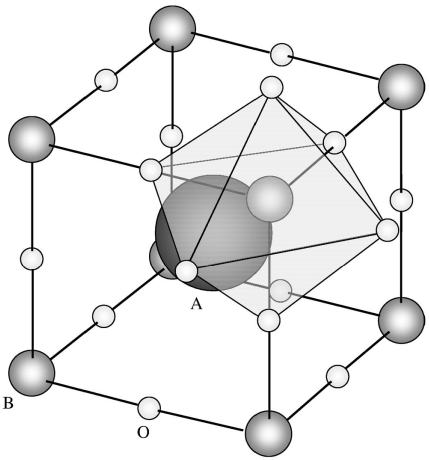
\includegraphics[scale=0.3]{fig/1-1.png}
\caption{钙钛矿结构ABO$_3$原胞及氧八面体示意图 \cite{ref2}.}
\label{fig:1-1} 
\end{figure}

一般地,A离子、B离子和O离子的半径大小满足关系
\begin{equation}
R_A+R_O=t\sqrt{2}(R_B+R_O).
\label{eq:1-1}
\end{equation}
其中$t$为容忍因子,对理想钙钛矿立方晶体$t = 1.00$;当$0.75 < t < 0.90$时,原胞中的原子半径不匹配,氧八面体无法竖直平行排列,由于畸变而呈正交结构.

%1.1.2
\subsection{钙钛矿结构过渡金属氧化物}
过渡金属元素原子的$d$轨道壳层未填满电子,在元素周期表中处在$d$壳层全空的碱土金属 (Ca, Sr, Ba) 和$d$壳层全满的贵金属 (Cu, Ag, Au) 之间,如图 \ref{fig:1-2}所示.

\begin{figure}[htbp]
\centering
\includegraphics[scale=0.5]{fig/1-2.png}
\caption{元素周期表 \cite{ref3}.}
\label{fig:1-2} 
\end{figure}

$d$轨道量子数$l = 2$,轨道角动量共有$(2l+1) = 5$个不同取向,不考虑自旋时,这5个轨道能量相同,对应的本征态波函数以球谐函数分别表示为
  $$Y_2^0=\frac{1}{4}\sqrt{\frac{5}{\pi}}(3\cos^2\theta-1)=\frac{1}{4}\sqrt{\frac{5}{\pi}}\frac{3z^2-r^2}{r^2},$$
  
  $$Y_2^{\pm 1}=\frac{-1}{2}\sqrt{\frac{15}{2\pi}}\sin\theta\cos\theta e^{\pm i\phi}=\frac{-1}{2}\sqrt{\frac{15}{2\pi}}\frac{(x\pm iy)z}{r^2},$$
  
  $$Y_2^{\pm 2}=\frac{1}{4}\sqrt{\frac{15}{2\pi}}\sin^2\theta e^{\pm 2i\phi}=\frac{1}{4}\sqrt{\frac{15}{2\pi}}\frac{(x\pm iy)^2}{r^2}.$$
以上五个本征态简并,通过线性组合可以得到实数形式波函数为
$$d_{z^2}=Y_2^0=\frac{1}{4}\sqrt{\frac{5}{\pi}}(3\cos^2\theta-1)=\frac{1}{4}\sqrt{\frac{5}{\pi}}\frac{3z^2-r^2}{r^2},$$
  
  $$d_{zx}=\frac{1}{2}(Y_2^1+Y_2^{-1})=\frac{-1}{2}\sqrt{\frac{15}{2\pi}}\sin\theta\cos\theta\cos\phi=\frac{-1}{2}\sqrt{\frac{15}{2\pi}}\frac{xz}{r^2},$$
  
  $$d_{yz}=\frac{1}{2i}(Y_2^1-Y_2^{-1})=\frac{-1}{2}\sqrt{\frac{15}{2\pi}}\sin\theta\cos\theta\sin\phi=\frac{-1}{2}\sqrt{\frac{15}{2\pi}}\frac{yz}{r^2},$$
    
  $$d_{x^2-y^2}=\frac{1}{2}(Y_2^2+Y_2^{-2})=\frac{1}{4}\sqrt{\frac{15}{2\pi}}\sin^2\theta\cos(2\phi)=\frac{1}{4}\sqrt{\frac{15}{2\pi}}\frac{x^2-y^2}{r^2},$$
  
  $$d_{xy}=\frac{1}{2i}(Y_2^2-Y_2^{-2})=\frac{1}{4}\sqrt{\frac{15}{2\pi}}\sin^2\theta\sin(2\phi)=\frac{1}{4}\sqrt{\frac{15}{2\pi}}\frac{2xy}{r^2}.$$

利用Python画出波函数的空间分布,如图 \ref{fig:1-3}所示,各个分布都具有特殊取向.

\begin{figure}[htbp]
\centering
\includegraphics[scale=0.5]{fig/1-3.png}
\caption{$d$轨道电子波函数空间分布.}
\label{fig:1-3} 
\end{figure}

在过渡金属钙钛矿氧化物ABO$_3$中,如果B元素是过渡金属元素,由于钙钛矿结构中存在以B金属离子为几何中心的氧八面体,对B金属离子而言则形成了一个八面体晶体场,打破了球对称性,如图 \ref{fig:1-4}(a)所示. 假设氧八面体中六个氧离子都位于$x$轴、$y$轴和$z$轴上,由于$d_{z^2}$轨道取向为$z$轴,$d_{x^2-y^2}$轨道取向为$x$轴和$y$轴,电子在这些取向上概率密度较大,因此处于氧八面体晶体场中时$d_{z^2}$和$d_{x^2-y^2}$轨道的电子受到氧离子的Coulomb排斥,导致能量升高;$d_{zx}$轨道、$d_{yz}$轨道和$d_{xy}$轨道的电子主要分布在坐标轴之间,避开了氧离子,能量相对较低,最终原本简并的五个能级在晶体场作用下发生劈裂. 

根据群论中正八面体$O_h$点群的特征标表,查得$d_{z^2}$和$d_{x^2-y^2}$是不可约表示$E_g$的基函数,$d_{zx}$、$d_{yz}$和$d_{xy}$是不可约表示$T_{2g}$的基函数,这两类本征态分别属于两个不同的不可约表示,能量一般不简并. 因此,对称性降低后高维不可约表示劈裂为多个低维不可约表示,具体地,$d$轨道在氧八面体晶体场下劈裂为一个二重简并的$E_g$轨道和一个三重简并$T_{2g}$轨道 \cite{ref5},如图 \ref{fig:1-4}(b)所示.

$$d=E_g\oplus T_{2g}$$

\begin{figure}[htbp]
\centering
\includegraphics[scale=0.8]{fig/1-4.png}
\caption{(a) 八面体晶体场(黑色点表示氧原子);\\(b) 3$d$轨道电子能级在八面体晶体场中能级劈裂\cite{ref4}.}
\label{fig:1-4} 
\end{figure}

以上分析表明,钙钛矿结构的过渡金属氧化物的电子结构比较复杂,电子与电子之间Coulomb相互作用不可忽略,属于强关联体系. 此外,部分过渡金属元素$d$壳层电子根据所受势场变化会发生能级跃迁,从而改变元素的价态. 由于电子之间的关联性,我们可以通过设计特殊的晶格结构或利用不同材料之间晶体场的差异调节电子的结构,材料中电荷、晶格、电子轨道、电子自旋等自由度互相协作、竞争,呈现崭新的现象. 本课题主要研究钙钛矿结构过渡金属氧化物界面中的二维电子气.

%1.2
\section{界面二维电子气}
1996年,Bell实验室一位年轻的物理学家Harold Hwang向当时的实验室主任 Horst St$\ddot{\mathrm{o}}$rmer提出要研究氧化物的异质界面体系,这在当时是一个全新的方向 \cite{ref6}. St$\ddot{\mathrm{o}}$rmer 是半导体薄膜的专家,和崔琦等合作者共同发现了分数量子霍尔效应,经验丰富的他认为Hwang的想法操作难度非常大,因为界面体系的新现象对实验得到的样品要求非常苛刻:薄膜需要相当平整、具有非常完美的单晶结构、且没有缺陷,这样电子才能不受非本征影响地传输并表现出新的性质,而St$\ddot{\mathrm{o}}$rmer团队也花了十几年时间才摸索出最佳实验条件. 然而Hwang没有气馁,终于生长得到了高质量的单晶氧化物薄膜,并于2004年和合作者共同发现LaAlO$_3$/SrTiO$_3$氧化物异质界面体系存在具有高迁移率的二维电子气 \cite{ref7},如图 \ref{fig:1-5}所示. 

\begin{figure}[htbp]
\centering
\includegraphics[scale=0.55]{fig/1-5.png}
\caption{(a) LaAlO$_3$/SrTiO$_3$体系高能电子衍射 (RHEED) 振荡;(b) LaAlO$_3$/SrTiO$_3$界面体系;(c) LaAlO$_3$/SrTiO$_3$体系方块电阻随温度变化曲线 \cite{ref7}.}
\label{fig:1-5} 
\end{figure}

值得注意的是,两种钙钛矿氧化物LaAlO$_3$和SrTiO$_3$都是能带绝缘体,带隙分别为 \SI{5.6}{eV}和 \SI{3.2}{eV} \cite{ref7};而它们形成的界面却是导体,表明界面的形成让对称性发生破缺,电子之间的强关联效应凸显,电子结构发生变化,从而出现体材料所没有的导电性. 这一现象的内部机制大致有三个机制:“极化不连续”导致电荷重构;氧空位缺陷的形成;界面原子扩散交换.

%1.2.1
\subsection{“极化不连续”理论}
为了解释LaAlO$_3$/SrTiO$_3$氧化物异质界面体系中二维电子气的形成,Hwang等人提出了“极化不连续”理论 \cite{ref8}. 如图 \ref{fig:1-6} (a, b) 所示,实验中LaAlO$_3$/SrTiO$_3$异质结构是利用脉冲激光沉积法外延生长得到,选择晶向为(001)的SrTiO$_3$衬底外延生长LaAlO$_3$薄膜,根据衬底的终端面的不同,界面的结构有两种可能情况:(a) n型:(Al$^{3+}$O$_2^{4-}$)$^-$/(La$^{3+}$O$^{2-}$)$^+$/(Ti$^{4+}$O$_2^{4-}$); (b) p型: (La$^{3+}$O$^{2-}$)$^+$/(Al$^{3+}$O$_2^{4-}$)$^-$/(Sr$^{2+}$O$^{2-}$). 其中LaAlO$_3$是极化晶体,每一层带有电荷;SrTiO$_3$是非极化晶体,每一层均为电中性. 如果不发生电荷转移,根据静电学平衡可知随着LaAlO$_3$薄膜原子层数增加,电势将单调增加从而导致发散,形成“极化灾难”.

\begin{figure}[htbp]
\centering
\includegraphics[scale=0.47]{fig/1-6.png}
\caption{(a, b) LaAlO$_3$/SrTiO$_3$异质结构两种界面可能情况及对应的“极化灾难”;\\
(c, d) LaAlO$_3$/SrTiO$_3$异质结构界面电荷转移 \cite{ref8}.}
\label{fig:1-6} 
\end{figure}

“极化灾难”在现实中不会发生,如图 \ref{fig:1-6} (c, d) 所示,在界面处会发生“电荷转移”. 在n型界面中,过渡金属层(Ti$^{4+}$O$_2^{4-}$)是衬底的终端,部分Ti元素从+4价变成+3价,发生电子重构,使该层带负电,从而避免了电势发散;而电子重构导致在界面处产生巡游电子,从而形成可导电的界面. 在p型界面中,终端层(Sr$^{2+}$O$^{2-}$)中的元素无法变价,但可以通过氧空位缺陷使该层带正电,从而避免电势发散;与n型界面不同的是,p型界面没有巡游电子的引入,故界面并不导电,这也与实验的结果相符 \cite{ref8}.

“极化不连续”理论能够解释大部分过渡金属氧化物异质界面的二维电子气现象,且可以解释实验中的临界尺寸效应,即薄膜超过一定层数时才会导电;由此,“电荷转移”对界面二维电子气的贡献得到了广泛的认同 \cite{ref9}.

%1.2.2
\subsection{界面二维电子气的其它解释}
另一个对界面二维电子气的解释是“氧空位缺陷”理论. 在生长钙钛矿氧化物薄膜时,一般采用脉冲激光沉积法,利用高能脉冲激光对靶材的轰击形成等离子体羽辉,逐层沉积到衬底上;而这一过程中羽辉也会对衬底的晶格带来冲击,导致氧空位缺陷的产生. 对n型界面,每个氧空位将释放两个电子,相当于n型掺杂,导致界面上载流子浓度增强. 在实验上也观测到,随着生长条件氧压的增加,LaAlO$_3$/SrTiO$_3$异质界面的电阻增大,Hall迁移率显著减小,如图 \ref{fig:1-7}所示 \cite{ref10}. 这些事实都表明氧空位缺陷在界面二维电子气中也起到重要的作用.

\begin{figure}[htbp]
\centering
\includegraphics[scale=0.5]{fig/1-7.png}
\caption{(a) 不同生长氧压下 LaAlO$_3$/SrTiO$_3$界面电阻随温度变化曲线;\\
(b) LaAlO$_3$/SrTiO$_3$界面Hall迁移率随生长氧压的变化 \cite{ref10}.}
\label{fig:1-7} 
\end{figure}

另外,对LaAlO$_3$/SrTiO$_3$异质界面的扫描透射电镜研究表明,在界面处原子之间有明显的“混杂”,如图 \ref{fig:1-8}所示,在衬底中有La原子掺杂,形成导电层,这也可能是导致界面二维电子气产生的原因 \cite{ref11}.

\begin{figure}[htbp]
\centering
\includegraphics[scale=0.45]{fig/1-8.png}
\caption{(a) LaAlO$_3$/SrTiO$_3$界面少量原子掺杂理论图示;\\ 
(b) LaAlO$_3$/SrTiO$_3$界面扫描电镜-电子能量损失能谱结果 \cite{ref11}.}
\label{fig:1-8} 
\end{figure}

%1.3
\section{异质界面体系新奇物性}
继Hwang发现LaAlO$_3$/SrTiO$_3$异质界面二维电子气后,对钙钛矿过渡金属氧化物异质界面的研究吸引了人们的注意,大家开始寻找类似的体系,希望寻找这种异质界面体系的特征和物理根源,同时这个体系也是研究低维电输运、强关联电子体系的良好平台.
 
对于异质界面体系的生长,如果要得到良好的晶体薄膜,靶材和衬底的晶格常数需要满足一定条件,即不能差别太大,否则界面处无法匹配. 一般地,薄膜晶格常数$a_{\mathrm{film}}$与衬底晶格常数$a_{\mathrm{sub}}$不完全相等,用晶格失配度$\delta$描述其差别:

\begin{equation}
\delta=\frac{a_{\mathrm{film}}-a_{\mathrm{sub}}}{a_{\mathrm{sub}}}
\label{eq:1-5}
\end{equation}

若晶格失配度过大,薄膜将会受到应力,也有可能会产生较多缺陷,导致难以获得单晶薄膜. 一些常见的金属氧化物的晶格常数如图\ref{fig:1-9}所示 \cite{ref12}.

\begin{figure}[htbp]
\centering
\includegraphics[scale=0.5]{fig/1-9.png}
\caption{常见金属氧化物晶格常数比较 \cite{ref12}.}
\label{fig:1-9} 
\end{figure}

%1.3.1
\subsection{界面超导}
超导体是特殊的导体,具有两个特征:在超导转变温度$T_c$以下,超导体电阻率为零,即零电阻现象;处于磁场中时,超导体内部磁感应强度为零,即完全抗磁性. 当外磁场增大到临界磁场$H_c$,或当通过超导体的电流密度增大到临界电流密度$J_c$时,超导体将从超导态转变为正常态. 这些临界阈值越大,越有利于实际应用.

超导电性最初于1911年由H. K. Onnes在汞中发现,超导转变温度为 \SI{4.2}{K}. 人们开始寻找超导材料,同时也出现了许多尝试解释超导电性的理论模型,如London 方程、Ginzburg-Landau模型等 \cite{ref16},其中由美国物理学家J. Bardeen、L. N. Cooper 和J. R. Schrieffer三人共同提出的BCS理论 \cite{ref17}能够解释大多超导体的超导电性:对于电子与晶格作用强的材料,在低温条件下两个自旋相反的电子通过交换声子的方式进行配对形成Cooper对,从而在晶格中无耗散运动形成超导电流. 

在BCS理论框架下,超导电性起源于电子-声子相互作用,超导材料的临界阈值如超导转变温度$T_c$主要由载流子浓度、Debye温度以及电子-声子相互作用强度决定 \cite{ref18},其中Debye温度主要反映低温下声子的激发情况. 然而,许多材料要么Debye温度过低,要么载流子浓度过低,导致很难出现超导电性;如果通过人工构建不同材料的异质界面,界面共享两侧材料的特性,从而可能同时满足具有较高的载流子浓度和较高的Debye温度,增强电子-声子相互作用,从而有助于超导电性的出现. 因此,界面超导这一想法被研究者们关注,并借助半导体工艺中的原子层沉积技术开始在实验层面上设计、搭建异质界面体系,如La$_2$CuO$_4$/LaSrCuO$_4$ \cite{ref19}、FeSe/SrTiO$_3$ \cite{ref20}等体系. 

2007年,N. Reyren等人首次发现钙钛矿过渡金属氧化物异质界面LaAlO$_3$/SrTiO$_3$ 的超导迹象,如图 \ref{fig:1-10}所示,界面的超导转变温度约 \SI{200}{mK} \cite{ref15},极大地鼓舞了人们研究界面超导的热情.

\begin{figure}[htbp]
\centering
\includegraphics[scale=0.5]{fig/1-10.png}
\caption{LaAlO$_3$/SrTiO$_3$界面超导. (A) 方块电阻随温度变化的曲线;(B) 不同垂直磁场下方块电阻随温度变化的曲线;(C) 上临界磁场$H_{c2}$随温度变化的曲线[15].}
\label{fig:1-10} 
\end{figure}

%1.3.2
\subsection{基于KTaO$_3$的界面超导}
钽酸钾KTaO$_3$是另一种常见的钙钛矿过渡金属氧化物,与SrTiO$_3$不同的是, KTaO$_3$中Ta的外层电子为$5d$轨道电子,自旋轨道耦合效应更明显. 实验上,在以 KTaO$_3$ 为衬底构造的异质界面体系 (a-LaAlO$_3$/KTaO$_3$ \cite{ref13}, LaTiO$_3$/KTaO$_3$ \cite{ref14}) 中也发现有二维电子气的形成. 随着对KTaO$_3$的进一步探索,研究者们还发现了与 LaAlO$_3$/SrTiO$_3$ 体系类似的界面超导现象,如图 \ref{fig:1-11}所示,a-LaAlO$_3$/KTaO$_3$(110)的超导转变温度$T_c$达到 \SI{0.9} {K} \cite{ref21},a-LaAlO$_3$/KTaO$_3$(111)的$T_c$可达\SI{1.47} {K} \cite{ref22},另外 EuO/KTaO$_3$(111)的$T_c$可达 \SI{2.2}{K} \cite{ref22} ,比LaAlO$_3$/SrTiO$_3$体系界面超导转变温度高一个量级.

\begin{figure}[htbp]
\centering
\includegraphics[scale=0.6]{fig/1-11.png}
\caption{高角环形暗场像-扫描电子显微镜结果及超导零电阻现象. \\(a, b) a-LaAlO$_3$/KTaO$_3$ (110) 界面 \cite{ref21};(c, d) EuO/KTaO$_3$ (111) 界面 \cite{ref22}.}
\label{fig:1-11} 
\end{figure}

另外,研究者们还发现在EuO/KTaO$_3$ (111) 样品的输运测量实验中发现面内各向异性 \cite{ref22},如图 \ref{fig:1-12}所示,当温度下降至 \SI{2.2}{K} 时,沿不同方向的电阻随温度变化趋势不同,形成“条纹相” (stripe phase),表明在EuO/KTaO$_3$ (111) 界面的电输运实验中出现面内各向异性.

\begin{figure}[htbp]
\centering
\includegraphics[scale=0.35]{fig/1-12.png}
\caption{(A) EuO/KTaO$_3$ (111) 面内电输运随温度变化各向异性及“条纹相”的产生;\\(B) 各向异性测量方向图示(以[1$\bar{1}$0]为例) \cite{ref22}.}
\label{fig:1-12} 
\end{figure}

\section{本章小结}
本章粗略介绍了强关联电子体系中钙钛矿过渡金属氧化物中的界面二维电子气现象,关注了以KTaO$_3$作为衬底的界面体系中的研究情况. 氧化物异质界面体系是当前凝聚态物理学研究的前沿热点,其中关于界面超导电性的研究可为非常规超导电性的产生机制提供重要线索,还为探索具有更高超导转变温度的新型界面超导体提供新的科学依据. 此外,界面本身是一种器件,对其电子气的研究可以为超导量子计算等潜在应用打好硬件基础. 本课题的工作主要聚焦于LaGaO$_3$/KTaO$_3$异质界面体系的制备及其电学输运特性的研究,一方面LaGaO$_3$与 KTaO$_3$的晶格常数匹配相对较好;另一方面KTaO$_3$中Ta中的电子具有较强的自旋-轨道耦合效应,因此可能会呈现出新奇的量子物性. 


%chapter 2
\chapter{实验仪器、原理和操作}
%2.1
\section{总技术路线}
钙钛矿过渡金属氧化物在异质界面体系可能会有新奇的物性出现,本毕业论文主要研究LaGaO$_3$/KTaO$_3$这一具体体系,在实验上主要包括两个部分:样品的制备,样品物性的表征. 其中,在LaGaO$_3$/KTaO$_3$体系样品制备中,由于在调研过程中未发现有其他研究者对该体系的生长经验,因此在生长薄膜前需要对生长条件进行摸索,探究不同生长条件下对样品性质的影响,找到最佳条件并进行新奇物性的探索. 在此基础上,结合原子力显微镜、X射线衍射、低温电输运测量等多种物性表征手段对最佳质量下的样品进行表征测试,并分析特点. 实验技术路线如图 \ref{fig:2-1}所示.

\begin{figure}[htbp]
\centering
\includegraphics[scale=0.5]{fig/2-1.pdf}
\caption{总技术路线.}
\label{fig:2-1} 
\end{figure}

在技术路线中,“摸索薄膜生长条件”中也需要通过初步的物性表征判断样品质量好坏. 本章节将粗略介绍在实验过程中使用的仪器,包括原理和操作.
%2.2
\section{脉冲激光沉积系统 (PLD)}
薄膜样品的制备方法有许多,主要分为化学气相沉积法 (Chemical Vapor Deposition, CVD) 和物理气相沉积法 (Physical Vapor Deposition, PVD). 本课题在复杂氧化物薄膜的生长中,选用脉冲激光沉积法 (Pulsed Laser Deposition, PLD) 构建LaGaO$_3$/KTaO$_3$异质界面体系,主要仪器为凯柏科技有限公司(台湾)的超高真空脉冲激光镀膜系统(型号PLD-12,如图 \ref{fig:2-2} (a) 所示)以及美国Coherent公司的脉冲激光光源(型号COMPex 102F,如图 \ref{fig:2-2} (b) 所示).

\begin{figure}[htbp]
\centering
\includegraphics[scale=0.6]{fig/2-2.png}
\caption{(a) 脉冲激光沉积系统实验仪器(局部);(b) 脉冲激光光源.}
\label{fig:2-2} 
\end{figure}

脉冲激光沉积法是一种常见的薄膜生长技术,利用高能量的脉冲激光轰击靶材,使靶材蒸发并沉积在衬底表面上形成薄膜,过程如图 \ref{fig:2-3}所示. 

\begin{figure}[htbp]
\centering
\includegraphics[scale=0.7]{fig/2-3.png}
\caption{脉冲激光沉积法流程示意图 \cite{ref23}.}
\label{fig:2-3} 
\end{figure}

在沉积过程中,衬底与靶材相对摆放. 脉冲激光束由准分子激光器提供,其中KrF气体为增益介质,激光波长 \SI{248}{nm},控制激光能量密度在 \SI{1}{J/cm^2}-\SI{5}{J/cm^2}范围内,每一下激光脉冲可以使一小部分靶材蒸发,蒸发出的靶材是等离子体,以羽辉的形式呈倒锥形喷射并沉积到衬底上. 整个过程大致可分成四步:\\
(1) 入射脉冲激光轰击靶材. 激光穿透靶材表面,穿透深度与激光波长、靶材吸收系数有关.\\
(2) 靶材蒸发形成等离子体. 靶材中电子被激光激发而振动,能量传递给晶格,靶材被迅速加热而蒸发.\\
(3) 等离子体沿靶材表面的法向扩散运动,形成羽辉. 这一过程与PLD腔内气体有关,气体与等离子体的相互作用会影响等离子体的扩散.\\
(4) 靶材物质沉积在衬底上,逐层堆积,薄膜生长. 这一过程是薄膜生长质量的关键,能量过大的等离子体与衬底接触时可能会发生强烈的冲击,从而在界面处形成缺陷;受冲击而被弹离原位的原子团再与等离子体接触,可能会在衬底上形成颗粒物.

由于激光能量源与真空腔体是分离的,脉冲激光沉积系统的装置调整自由度较高,且可以通过控制激光的脉冲数量来控制沉积薄膜的厚度,通过控制激光的脉冲频率来调整薄膜生长速率. 另外,靶材受到脉冲激光轰击时按照化学计量比蒸发,薄膜成分与靶材相同,因此脉冲激光法在生长金属氧化物薄膜或其他复合元素材料的薄膜中具有很大优势.

但是,脉冲激光沉积法也有一定的缺点. 因为等离子体的喷射过程,薄膜表面上可能会出现较多的颗粒状生长. 为了避免这种颗粒状生长,应该选用质地较硬、表面较平整的靶材. 等离子体与衬底表面碰撞的过程有可能导致晶体缺陷的产生,而等离子体羽辉内部在不同角度上的能量分布不均则可能导致薄膜生长具有各向异性. 同时,等离子体的扩散也有可能污染激光的入射窗口,进而影响脉冲激光的入射.

%2.3
\section{原子力显微镜 (AFM)}
我们采用美国Oxford仪器公司生产的原子力显微镜(型号MFP-3D Classic,如图 \ref{fig:2-4}所示)探测衬底和薄膜样品表面的平整程度.

\begin{figure}[htbp]
\centering
\includegraphics[scale=0.4]{fig/2-4.png}
\caption{实验室中的原子力显微镜.}
\label{fig:2-4} 
\end{figure}

原子力显微镜 (Atomic Force Microscopy, AFM) 主要工作原理 \cite{ref24}是通过测量探针针尖与样品表面之间的相互作用力(van der Waals力),来显示出样品表面的起伏情况. 根据Hooke定律,针尖与表面间相互作用力可通过探针 (Tip) 所在的悬臂 (Cantilever) 的弯曲程度探测,而后者的微小弯曲位移通过光学技术进行测量,如图 \ref{fig:2-5}所示. 

针尖与样品表面间作用力与距离有关,如图 \ref{fig:2-6}所示,可根据相互作用力的排斥与吸引将AFM探测模式分为三种:接触模式 (contact mode), 非接触模式 (non-contact mode) 以及敲击模式 (tapping mode). 接触模式中,针尖与表面距离非常近,针尖受到表面的排斥力从而探测表面的起伏,优点是便于探测粗糙程度小的样品,而缺点则是探测过程可能损坏样品,不适合探测较软的样品;在非接触模式中,针尖与表面距离较远,约十至几百埃,针尖受到吸引力,悬臂在其共振频率附近作小范围振动,来自表面的吸引力则会影响振动的情况从而实现对表面的探测,优点是能够探测较软的样品,纵向精度能达到亚原子级别,缺点则是横向精度差,容易受环境影响;在敲击模式中,针尖与表面距离随悬臂在共振频率附近振动而变化,相互作用力时而排斥时而吸引,可以看做是前两种模式的结合,通过测量振动频率和相位的变化来显示样品表面的情况,消除了接触模式中的摩擦力,也避免了非接触模式中容易受环境影响的缺点. 因此,我们一般选用敲击模式测量样品表面的平整程度.

\begin{figure}[htbp]
\centering
\includegraphics[scale=0.5]{fig/2-5.png}
\caption{原子力显微镜测量样品表面起伏示意图 \cite{ref24}.}
\label{fig:2-5} 
\end{figure}

\begin{figure}[htbp]
\centering
\includegraphics[scale=0.5]{fig/2-6.png}
\caption{原子力显微镜三种测量模式示意图 \cite{ref24}.}
\label{fig:2-6} 
\end{figure}

%2.4
\section{X射线衍射 (XRD) 和X射线反射 (XRR)}
我们利用X射线衍射 (X-Ray Diffraction, XRD) 探测薄膜样品的结构,利用X射线反射 (X-Ray Reflection, XRR) 来测量薄膜的厚度. 在薄膜结构表征中常用X射线波长为 \SI{0.5}{Å}-\SI{2.0}{Å} \cite{ref25}. 对于特征X射线,当高速运动电子与物质相碰时,高速电子把原子内层电子轰出,外层电子跃迁进入内层空位,以X射线的形式向外释放能量,这类X射线波长与物质种类有关. 电子从原子L层轨道跃迁至$K$层空位,发出的X射线称为$K_\alpha$射线. 实验中选用铜靶,使用双晶单色仪后X射线波长为 \SI{1.5418}{Å}. 我们的实验仪器是德国Bruker公司生产的多功能X射线衍射仪(型号D8 Discover,如图\ref{fig:2-7}所示).

\begin{figure}[htbp]
\centering
\includegraphics[scale=0.4]{fig/2-7.png}
\caption{多功能X射线衍射仪.}
\label{fig:2-7} 
\end{figure}

晶体由原子或原子团按一定规律周期性排列而成,形成三维衍射光栅,当入射X射线的波长与晶格常数相近时,X射线衍射效应显著,可以通过探测X射线的衍射现象来探测晶体结构.

设入射X射线波矢为$\vec{k}$,出射X射线波矢为$\vec{k}'$,其中经过样品时X射线感受到的势场为$V(\vec{r})$,则跃迁矩阵元可以写成:

\begin{equation}
\langle \vec{k}'|V|\vec{k}\rangle=\int\mathrm{d}\vec{r}\frac{e^{-i\vec{k}'\cdot\vec{r}}}{\sqrt{L^3}}V(\vec{r})\frac{e^{i\vec{k}\cdot\vec{r}}}{\sqrt{L^3}}=\frac{1}{L^3}\int\mathrm{d}\vec{r}e^{-i(\vec{k}'-\vec{k})\cdot\vec{r}}V(\vec{r}).
\label{eq:2-1}
\end{equation}
 
而晶体中存在周期势场,其中$\vec{R}$为基矢或基矢的线性组合:

\begin{equation}
V(\vec{r})=V(\vec{r}+\vec{R}).
\label{eq:2-2}
\end{equation}

式子 (\ref{eq:2-1})中的积分可以写成对原胞的积分再求和:

\begin{equation}
\langle \vec{k}'|V|\vec{k}\rangle=\frac{1}{L^3}\int\mathrm{d}\vec{r}e^{-i(\vec{k}'-\vec{k})\cdot\vec{r}}V(\vec{r})=\frac{1}{L^3}\sum_{\vec{R}}\int_{unit-cell}\mathrm{d}\vec{x}e^{-i(\vec{k}'-\vec{k})\cdot(\vec{x}+\vec{R})}V(\vec{x}+\vec{R}).
\label{eq:2-3}
\end{equation}
计算得到
\begin{equation}
\langle \vec{k}'|V|\vec{k}\rangle=\frac{1}{L^3}\Big[\sum_{\vec{R}}e^{-i(\vec{k}'-\vec{k})\cdot\vec{R}}\Big]\Big[\int_{unit-cell}\mathrm{d}\vec{x}e^{-i(\vec{k}'-\vec{k})\cdot\vec{x}}V(\vec{x})\Big].
\label{eq:2-4}
\end{equation}
式子 (\ref{eq:2-4})当且仅当满足Laue方程时非零,即倒格矢$\vec{G}$满足$\vec{k}'-\vec{k}=\vec{G}$,
\begin{equation}
|\vec{k}|=|\vec{k}'|=\frac{2\pi}{\lambda}.
\label{eq:2-5}
\end{equation}
式子 (\ref{eq:2-5})称为Laue条件,实际上表示X射线在晶格散射中的动量守恒和能量守恒. Laue条件与Bragg定律等价,如图 \ref{fig:2-8}所示,X射线入射到晶格中发生布拉格散射,X射线在相邻晶格之间光程差满足Bragg条件时,出射X射线出现衍射极大,满足方程:
\begin{equation}
n\lambda = 2d\sin\theta.
\label{eq:2-6}
\end{equation}
其中$\lambda$为X射线波长,$n = 1, 2, 3, ...$为衍射级数.

\begin{figure}[htbp]
\centering
\includegraphics[scale=0.3]{fig/2-8.png}
\caption{晶体中的Bragg衍射示意图 \cite{ref26}.}
\label{fig:2-8} 
\end{figure}

在X射线衍射实验中,可以通过测量出射光强度随角度的变化,观察是否存在晶体衍射峰,根据对应的角度位置,确定晶格常数. 类似地,若已知晶体的晶格常数,可以计算得到衍射峰的位置,通过X射线衍射实验的测量观察是否薄膜样品是否存在单晶相.

而在X射线反射实验中,通过测量薄膜样品对X射线的反射率来计算薄膜厚度. 当入射X射线以与薄膜表面夹角很小的角度入射时,X射线在薄膜上表面和薄膜与衬底之间的界面发生反射,形成两束反射X射线. 当薄膜厚度$d$满足Bragg条件 (\ref{eq:2-6})时,反射X射线干涉相长,强度达到极大. 记录极大值对应夹角$\theta_m$和相应的衍射级数$n$,考虑半波损失和修正$\delta$后有\cite{ref27, ref28}:
\begin{equation}
\sin^2\theta_m = \frac{\lambda^2}{4d^2}(n+\delta n)^2+\delta.
\label{eq:2-7}
\end{equation}
由于电磁波从波疏介质到波密介质的反射存在半波损失. 若薄膜密度大于衬底密度,则 $\delta n = 1/2$;若薄膜密度小于衬底密度,则$\delta n = 0$. 对$\sin2\theta_m$关于$(n+\delta n)^2$作线性拟合,即可在斜率参数中获得薄膜厚度的信息.

%2.5
\section{透射电子显微镜 (TEM)}
20世纪初,物理学家们发现了实物粒子也具有波动性,比如电子波长可以根据Louis de Broglie关系计算得
\begin{equation}
\lambda = \frac{h}{p} = \frac{h}{mv},
\label{eq:2-8}
\end{equation}
其中Planck常数 $h = \SI{6.626e-34}{J\cdot s}$,$p$为电子的动量. 从加热灯丝或场发射源出射到真空中的电子,受到 \SI{50}{V}的加速电压时速度 $v\approx\SI{4.2e6}{m/s}$,相应的波长 $\lambda\approx\SI{0.17}{nm}$,这一波长接近原子尺度,因此这类电子可用于探测晶体表面的结构. 当加速电压提高到 \SI{50}{kV}时,电子波长约\SI{5}{pm},这类高能电子在固体中穿透深度可达几微米. 在透射电子显微镜 (transmission electron microscope, TEM) 中,聚焦的高能电子穿过较薄的样品发生弹性散射,经探测器处理后得到电子衍射谱,可以得到晶体的周期性结构,其分辨率远远超过光学显微镜 \cite{ref29}. 

入射电子与材料相互作用还可能发生非弹性散射,能量可被材料吸收. 材料中内壳层的电子被激发而出射,称为次级电子 (secondary electrons). 外壳层电子跃迁进入内壳层,以特征X射线的方式释放能量. 与透射电镜类似,扫描电子显微镜 (scanning electron microscope, SEM) 用电子束扫描样品,并用探测器收集从材料出射的电子、特征X射线等信号,即可得到材料表面的结构、元素等信息.
 
扫描透射电子显微镜 (scanning transmission electron microscope, STEM) 是一种结合了扫描电子显微镜特点的透射电子显微镜,如图 \ref{fig:2-9}所示,从场发射电子枪出射的电子聚焦成原子尺度的电子束斑在样品上,通过扫描线圈控制电子束斑进行扫描,样品下方的环形探测器用于接收被散射的电子 \cite{ref30}. 不同角度位置的探测器探测的信号有所不同,在$\beta_1$范围内,探测器接收到透射电子和部分散射的电子,形成环形明场像 (annular bright field, ABF);而在$\beta_2$范围,探测器主要接收发生了Bragg散射的电子,形成环形暗场像 (annular dark field, ADF);而角度范围进一步扩大时,信号主要来自非相干散射电子,形成高角度环形暗场像 (high-angle annular dark field, HAADF). HAADF来自入射电子与材料原子$1s$态电子的散射,通常能够直接反应元素的信息. 另外,样品上方还可以放置一个X射线能谱仪探测材料内原子的特征X射线,形成X射线能谱 (energy diffraction spectra, EDS),得到不同元素在样品中的分布情况.

\begin{figure}[htbp]
\centering
\includegraphics[scale=0.6]{fig/2-9.png}
\caption{STEM成像原理示意图 \cite{ref30}.}
\label{fig:2-9} 
\end{figure}

%2.6
\section{Raman光谱 (Raman spectra)}
我们利用美国Horiba公司生产的高分辨Raman光谱仪(型号LabRAM HR Evolution,如图 \ref{fig:2-10}所示)测量薄膜样品的Raman光谱. 

\begin{figure}[htbp]
\centering
\includegraphics[scale=0.5]{fig/2-10.png}
\caption{实验室Raman光谱仪.}
\label{fig:2-10} 
\end{figure}

Raman散射最初由C. V. Raman于1928年在实验中发现. 当一束单色光投射到材料中时,光发生反射、透射、散射或被材料吸收. 对于光的散射过程,光作为入射电磁波诱导材料中的极化偶极子发生振荡,并对外辐射新的电磁波,与入射电磁波耦合后形成散射光. 若散射光频率与入射光频率相同,这种散射称为Rayleigh散射;若散射光频率与入射光频率不同,波数差别在\SI{1}{cm^{-1}}以上时,这种散射称为Raman散射,波数差称为Raman位移 (Raman shift).

从经典电磁学理论分析,材料中偶极矩的振动频率与其对外辐射频率相同. 入射电磁波使材料内部极化产生的偶极矩进行受迫振动,偏移平衡的位移大小记为$q(t)$,共振频率记为$\omega_q$,长时间的振动解为
$$q(t)=Q_0\cos(\omega_qt).$$
偶极矩的极化强度大小$P$与电场强度大小$E$有关,
$$P=\varepsilon_0\alpha E,$$
其中 $\varepsilon_0$为真空介电常数,极化率 $\alpha = \alpha(q)$可对位移$q$作Taylor展开,位移较小可忽略二阶及以上高阶项,
$$\alpha(q) = \alpha_0 + \frac{\mathrm{d}\alpha}{\mathrm{d}q}\Big|_{0}q + \frac{1}{2}\frac{\mathrm{d}^2\alpha}{\mathrm{d}q^2}\Big|_{0}q^2 + ... \approx \alpha_0 + \frac{\mathrm{d}\alpha}{\mathrm{d}q}\Big|_{0}q.$$
设电场强度$E$以频率$\omega_L$振荡,相位与偶极矩振动相位都为0,
$$E = E_0\cos(\omega_Lt).$$
偶极矩极化强度可以写成
\begin{align*}
  P &= \varepsilon_0\Big[\alpha_0 + \frac{\mathrm{d}\alpha}{\mathrm{d}q}\Big|_{0}Q_0\cos(\omega_qt)\Big]E_0\cos(\omega_Lt) \\
    &= \varepsilon_0\alpha_0E_0\cos(\omega_Lt)+\varepsilon_0\frac{\mathrm{d}\alpha}{\mathrm{d}q}\Big|_{0}E_0Q_0\cos(\omega_qt)\cos(\omega_Lt).
\end{align*}
可以看到第一项辐射频率等于电场频率,为Rayleigh散射项;第二项为Raman散射项,其中利用三角函数积化和差公式可得
$$\cos(\omega_qt)\cos(\omega_Lt)=\frac{1}{2}\Big[\cos(\omega_L+\omega_q)t+\cos(\omega_L-\omega_q)t\Big]$$
因此Raman散射的频率刚好等于电场振动频率与偶极矩共振频率的和或差. 频率为$\omega_L-\omega_q$的散射,称为Stokes散射;频率为$\omega_L+\omega_q$的散射,称为Anti-Stokes散射.

由于材料中偶极矩对入射电磁波的响应,对外辐射包括Rayleigh散射和Raman 散射,其中Raman位移与偶极矩的共振频率对应. 但从实验上,Stokes散射的强度总是大于Anti-Stokes散射的强度,这是经典分析所不能解释的. 

从量子力学分析,材料中的分子由于化学键而存在振动、转动能级,电子也存在能级;对于晶体而言,存在声子能级,这些量子化的能级以及能级差是材料的“指纹”信息. 当材料受到入射电磁波的激发时,材料内部的分子或电子吸收能量,体系从初态达到一系列能级的组合态(称为虚能级),从这一高能态返回到低能级时,由能量守恒,材料将对外辐射出特定波长的电磁波,这一特定波长对应的波数即Raman位移. 从低能级出发,最后落在较高能级时,这一辐射为Stokes散射;从较高能级出发,最终落在低能级时,这一辐射为Anti-Stokes散射. 

在二次量子化描述下,受激Raman散射理论给出跃迁几率与初态的粒子数有关 \cite{ref31},而在半经典描述下体系粒子数在不同能级上满足Boltzmann分布,位于低能级的粒子数大于位于高能级的粒子数,因此Stokes散射发生的概率大于Anti-Stokes散射,在实验中可以观测到频率减小的散射光强度大于对称的频率增大的散射光强度.

晶体是原子排列具有长程周期性的固体,其振动模式数量与原子数目有关,相应的元激发称为声子. 声子的振动也具有一定的能级,可以从外界吸收能量而跃迁到高能级,也可以对外辐射能量而落到低能级. 因此,这些具有周期性结构的晶体也可以发生Raman散射,Raman位移即对应着晶体的声子不同能级之间共振频率,是晶体的“指纹”信息,因此Raman光谱是对晶体进行表征、判断结晶情况好坏的重要光学手段. 一些常见的简单钙钛矿结构晶体的Raman光谱如图 \ref{fig:2-11}所示,可见不同结构的晶体具有不同的声子振动模式,振动频率不同,体现在Raman光谱中峰值对应的Raman位移不同.

\begin{figure}[htbp]
\centering
\includegraphics[scale=0.4]{fig/2-11.png}
\caption{一些钙钛矿晶体的Raman光谱 \cite{ref32}\\
(CZ: CaZrO$_3$; ST: SrTiO$_3$; CT: CaTiO$_3$; NA: NdAlO$_3$; LG: LaGaO$_3$).}
\label{fig:2-11} 
\end{figure}

%2.7
\section{低温电输运测量}
低温电输运测量是我们对薄膜样品的主要物性表征手段,对于LaGaO$_3$/KTaO$_3$ 界面体系,薄膜和衬底都是绝缘体,若形成界面体系后形成二维电子气,则样品具有导电性,这一导电性可能表现出崭新的物性,因此低温电输运测量在本实验中非常重要. 

如图 \ref{fig:2-12}所示,实验室中采用美国Oxford仪器公司生产的无液氦低温超导磁体系统,结合电流电压测量设备,可以测量不同温度下、不同磁场下样品的电阻变化. 该系统主要用于低温电学输运特性测试,测量温度变化范围:\SI{1.5}{K}-\SI{300}{K},磁场变化范围:\SI{0}{T}-\SI{12}{T}.

\begin{figure}[htbp]
\centering
\includegraphics[scale=0.5]{fig/2-12.png}
\caption{低温电输运测量系统.}
\label{fig:2-12} 
\end{figure}

无液氦低温系统的降温过程如图 \ref{fig:2-13} (a) 所示. 制冷部件 (PTR) 的主要作用是给磁体、样品制冷,给磁体制冷是为了让磁体处于其超导态,从而通过另一部件控制磁场的变化;而给样品制冷则是为样品提供低温环境. 高压氦气从红色通路进入体系,在\SI{4} {K}脉管制冷机中经过两次绝热膨胀先从室温(约\SI{300}{K})降温至\SI{50}{K},再下降到\SI{4}{K}液化;通过控制针阀 (Needle valve),可以使低温液氦流入样品腔侧壁,与样品腔侧壁发生热交换. 对液氦进行减压,液氦通过蒸发继续降温,根据液氦饱和蒸气压与沸点的关系(图 \ref{fig:2-13} (b)),蒸气压压强越小,随着液氦的蒸发后液态的氦温度越低,对于本实验室仪器主要降温介质为$^4$He,可降温至\SI{1.5}{K},更低气压时与样品腔侧壁热交换的$^4$He分子数目减少,增加液氦流入时反而使样品侧壁温度上升,因此存在温度最低阈值,对应一个最低气压,通常为\SI{2}{mbar}. 通过低压下液氦与侧壁的热交换,样品腔内环境可降到所需的温度. 吸收了系统热量后的气态$^4$He离开制冷机,再经过压缩机和水冷系统后重新成为高压氦气进入体系,形成一个闭循环,用于制冷的$^4$He不发生消耗,故称为“无液氦低温系统”.

\begin{figure}[htbp]
\centering
\includegraphics[scale=0.5]{fig/2-13.png}
\caption{ (a) 无液氦低温系统示意图;(b) He饱和蒸气压与沸点关系 \cite{ref33}.}
\label{fig:2-13} 
\end{figure}

%2.7.1
\subsection{van der Pauw法}
电输运性质是异质界面体系较常见的物性,第1章中提到的钙钛矿过渡金属氧化物异质界面体系中形成界面二维电子气,主要就是指电输运的特性.不同温度、不同磁场下的电阻变化,统称为电输运性质. 方块电阻 (sheet resistance) 是薄膜样品的特性,薄膜样品总电阻等于方块电阻与长宽比的乘积,方块电阻大小等于薄膜电阻率与薄膜厚度之比,其量纲为 $\Omega$,一般记为 $\Omega/\qedsymbol$. 
\begin{equation}
R_{\mathrm{sheet}}=\frac{\rho}{t},\quad R=R_{\mathrm{sheet}}\frac{L}{W}.
\label{eq:2-9}
\end{equation}
\begin{figure}[htbp]
\centering
\includegraphics[scale=0.5]{fig/2-14.png}
\caption{方块电阻.}
\label{fig:2-14} 
\end{figure}

测量方块电阻的常用方法是van der Pauw法 \cite{ref35}. 如图 \ref{fig:2-15} (a) 所示,对一块厚度为$d$的正方形薄膜样品,四个端点1、2、3、4作为与导线相连的接线口,其中两个端口通电流,另外两个端口测量电势差,四根导线所用的材料相同,以消除导线电阻和接触电阻的影响. 
\begin{figure}[htbp]
\centering
\includegraphics[scale=0.5]{fig/2-15.png}
\caption{(a) van der Pauw法测量示意图;(b) Hall效应 \cite{ref34}.}
\label{fig:2-15} 
\end{figure}

设$\rho$为样品电阻率,$d$为样品厚度,$I_{12}$为从端口1进入样品、从端口2离开样品的电流大小,$V_{34}=V_3-V_4$为端口3与端口4之间的电势差. van der Pauw法测量方法如下:分别测量跨阻 (trans-resistance) $R_{ij, kl}\equiv V_{kl}/I_{ij}$,
\begin{equation}
R_{12,43}\equiv\frac{V_{43}}{I_{12}},\quad R_{14,23}\equiv\frac{V_{23}}{I_{14}},\quad R_{21,34}\equiv\frac{V_{34}}{I_{21}},\quad R_{41,32}\equiv\frac{V_{32}}{I_{41}}.
\label{eq:2-10}
\end{equation}
van der Pauw法直接给出$R_{ij, kl}$与样品电阻率$\rho$、样品厚度$d$的关系 \cite{ref35}:
\begin{equation}
e^{-\frac{\pi d}{\rho}R_{12, 43}}+e^{-\frac{\pi d}{\rho}R_{14, 23}}=1.
\label{eq:2-11}
\end{equation}
定义$R_{\mathrm{vertical}}$和$R_{\mathrm{horizontal}}$满足:
\begin{equation}
R_{\mathrm{vertical}}=\frac{R_{12, 43}+R_{34, 12}}{2},\quad R_{\mathrm{horizontal}}=\frac{R_{23, 41}+R_{41, 23}}{2}.
\label{eq:2-12}
\end{equation}
可得到方块电阻$R_{\mathrm{sheet}}$满足方程
\begin{equation}
e^{-\pi R_{\mathrm{vertical}}/R_{\mathrm{sheet}}}+e^{-\pi R_{\mathrm{horizontal}}/R_{\mathrm{sheet}}}=1.
\label{eq:2-13}
\end{equation}

在实验中,利用恒流源和电压表结合Oxford低温超导磁体系统,测量$R_{ij, kl}$随温度或磁场的变化曲线,利用式子 (\ref{eq:2-13}) 解方程即可得到方块电阻随温度或磁场的变化曲线,数值上可利用Newton-Raphson方法求解. 

在磁场中,样品的电输运出现Hall效应和磁阻效应. 如图 \ref{fig:2-15} (b) 所示,载流子在磁场中运动时受到Lorentz力而偏移,导致样品在横向存在电势差,与磁场大小成正比,这就是Hall效应. 载流子受到Lorentz力而偏移,散射增加,在原电流方向上表现为电阻增加,这就是磁阻效应.

如图 \ref{fig:2-15} (b) 所示,假设在薄膜样品中通有纵向电流$I$,在垂直于样品所在平面的磁场作用下载流子偏转而导致存在电势差$V_H$,设载流子漂移速度为$v$,载流子体浓度为$n$,根据Lorentz力和电场力平衡有:
\begin{equation}
F=qvB=q\frac{V_H}{w},
\label{eq:2-14}
\end{equation}
\begin{equation}
I = nqSv,\quad S=dw.
\label{eq:2-15}
\end{equation}
则可得到横向“电阻”$V_H/I$和载流子面浓度$n_S$:
\begin{equation}
\frac{V_H}{I}=\frac{B}{nqd}=\frac{B}{n_Sq},\quad n_S=nd.
\label{eq:2-16}
\end{equation}

在van der Pauw法中,只要测量不同磁场$B$下$R_{13}$或$R_{24}$即可得到相应的变化曲线,通过线性拟合即可求出薄膜样品的载流子面浓度.

m型载流子(m = n 或p,n型表示载流子为电子,p型表示载流子为空穴)样品的电阻率可以表示为
\begin{equation}
\rho = \frac{1}{qn_m\mu_m},
\label{eq:2-17}
\end{equation}
其中$\mu_m$为载流子迁移率,根据方块电阻$R_{\mathrm{sheet}} = \rho/d$,可以求出薄膜样品的载流子迁移率:
\begin{equation}
\mu_m = \frac{1}{qn_SR_{\mathrm{sheet}}}.
\label{eq:2-18}
\end{equation}

%2.7.2
\subsection{Hall bar法}
为了测量薄膜样品在某一特定方向上的电输运性质,我们需要用Hall bar法,在样品表面上根据所需电流方向刻出图案,让电流在样品图案上沿特定方向流动,并在特定位置测量电压. 如图 \ref{fig:2-16}所示,白色区域是样品的有效测量区域,黑色实线为用光刻或其它方法使有效测量区域与灰色的无用区域隔绝. 实验中仅作粗略探索,没有使用光刻技术精细划分,而是在显微镜下手动用刻刀在样品表面刮出特定形状,被刮过的划痕电阻极大,相当于将薄膜的有效测量区域分离出来.

\begin{figure}[htbp]
\centering
\includegraphics[scale=0.5]{fig/2-16.png}
\caption{Hall bar法测量电阻示意图.}
\label{fig:2-16} 
\end{figure}

测量特定区域的薄膜电阻$R$、纵向长度$l$以及横向宽度$w$,即可根据式子 (\ref{eq:2-9}) 得到薄膜的方块电阻$R_{\mathrm{sheet}} = R\cdot w/l$. 类似地,若想测量薄膜样品的Hall效应,则在图 \ref{fig:2-16}中电流的接口不变,测量端口2与端口6之间的电势差即可得到相应的横向电压$V_H$,利用式子 (\ref{eq:2-16}) 和 (\ref{eq:2-18}) 即可分别求得载流子面浓度和载流子迁移率.

两种不同的方块电阻测量方法都适用于薄膜样品,van der Pauw法对薄膜样品的形状没有严格规定,只要样品厚度均匀、具有平面形状、没有孤立的空洞即可,此外还要求样品本身均匀、具有各向同性,四个电极需要在样品的边缘,电极与样品接触的面积远小于样品的面积. Hall bar法则对样品的有效形状有严格规定,一般需要进行微纳尺度的光刻加工. 两种方法测量方块电阻都不需要知道薄膜的具体厚度,其中Hall bar法需要知道有效性状的长度和宽度;测量Hall效应时,Hall bar法效果更好,因为电流方向控制较好,而van der Pauw法中电流沿着整个薄膜或界面流动. 此外,由于通电流与测量电压的导线不在同一个位置,两种方法都能有效避免接触电阻的影响,减小误差.

确定好薄膜的测量方法后,即可将样品粘贴在电路器件,用多功能微控楔键合机进行导线连接(一般用Al线),使样品作为一个元件参与电路,然后放入低温电学输运测量系统中测量.

\begin{figure}[htbp]
\centering
\includegraphics[scale=0.5]{fig/2-17.png}
\caption{电输运测量中的打线与测量}
\label{fig:2-17} 
\end{figure}

\section{本章小结}
本章介绍了研究LaGaO$_3$/KTaO$_3$异质界面体系的主要流程,包括样品的制备、样品的结构表征以及物性表征;粗略介绍了实验中使用的仪器、原理和操作. 制备LaGaO$_3$/KTaO$_3$异质界面薄膜样品的过程包括对衬底的处理、脉冲激光沉积过程,在摸索薄膜生长条件过程中利用原子力显微镜、X射线衍射和X射线反射等结构表征及时获得反馈,同时结合低温电输运测量检测薄膜生长的质量,从而及时调整生长条件,从而找到生长高质量薄膜的最佳条件. 



%chapter 3
\chapter{实验过程、数据和分析}
前两章节介绍了LaGaO$_3$/KTaO$_3$异质界面体系研究的背景和实验仪器的基本原理,本章节将讲述实验的过程、实验数据以及分析. 对钙钛矿过渡金属氧化物异质界面体系的研究从Hwang发现LaAlO$_3$/SrTiO$_3$界面二维电子气 \cite{ref7}就已经开始,后续有很多在其它氧化物界面上的研究,如LaGaO$_3$/SrTiO$_3$界面 \cite{ref36}、LaAlO$_3$/KTaO$_3$界面 \cite{ref21, ref45}、EuO/KTaO$_3$界面 \cite{ref22}等. 本课题的研究对象LaGaO$_3$/KTaO$_3$ (111) 界面未曾有过相关研究,属于探索性的课题. 课题虽然谈不上突破性的创新,仅仅是在不同体系中研究类似的现象,但对实验技能的要求较高,实验条件也需要实验者学习、摸索,而这也是笔者在毕业设计期间的主要工作. 

笔者先利用实验室的设备,学习实验上搭建异质界面体系的基本方法,主要通过构建LaAlO$_3$/SrTiO$_3$ (001) 异质界面体系来熟悉实验流程,同时希望能重复前人的实验结果. 在此之后,将开始摸索LaGaO$_3$/KTaO$_3$ (111) 界面体系的实验室条件,包括对衬底的处理、生长条件的探索、基本结构和物性的表征等. 最后,在获得最佳实验室条件后,对所生长的样品LaGaO$_3$/KTaO$_3$ (111) 界面进行物性表征和探究,主要包括二维电子气的形成、界面超导迹象的探索、面内电输运各向异性的探究等等.

%3.1
\section{LaAlO$_3$/SrTiO$_3$ (001) 异质界面体系}
LaAlO$_3$/SrTiO$_3$ (001) 界面可谓是过渡金属氧化物界面研究的先祖,最早由 Hwang等人于2004年制得高质量单晶氧化物薄膜,并发现具有高迁移率的二维电子气 \cite{ref7};随后对这一体系继续研究的人越来越多,发现了这一体系不仅具有导电性,还有磁性\cite{ref37}、界面超导\cite{ref15}等新奇物性,因此LaAlO$_3$/SrTiO$_3$ (001) 界面成了探索钙钛矿过渡金属氧化物异质界面新奇物性的典型平台. 这一研究的深入,也使得实验上制备LaAlO$_3$/SrTiO$_3$ (001) 界面的条件越来越成熟,实验时可参考前人的生长条件,结合实验室实际条件制备薄膜样品.

%3.1.1
\subsection{ SrTiO$_3$衬底的处理与LaAlO$_3$/SrTiO$_3$ (001) 的生长条件}
实验室使用合肥科晶材料技术有限公司生产的SrTiO$_3$ (001) 单晶衬底和LaAlO$_3$ 多晶靶材. 一般而言,从商业途径获得的单晶衬底表面存在一个微小的斜切角 (miscut angle),即实际晶面法向量与理想晶向之间的微小夹角,一般小于$\SI{0.1}{^\circ}$,导致衬底表面上的原子层种类混淆. 例如钙钛矿氧化物ABO$_3$在晶向[001]上由原子层AO和BO$_2$依次排列,由于存在斜切角,表面上既有AO成分又有BO$_2$成分,导致薄膜在制备时无法外延一层一层地生长,难以形成单晶. 因此,衬底必须经过处理才能使用,处理流程和处理结果如图 \ref{fig:3-1}所示 \cite{ref12}.
  
\begin{figure}[htbp]
\centering
\includegraphics[scale=0.7]{fig/3-1.png}
\caption{衬底处理流程;(a, b) 未处理的衬底结构和表面图;\\(c, d) 处理后的衬底结构和表面图 \cite{ref10}.}
\label{fig:3-1} 
\end{figure}

在笔者所在的实验室中,对衬底的处理流程大致如图 \ref{fig:3-2}所示,其中酸洗过程涉及剧毒物质氢氟酸和氟化铵溶液,该过程需要在通风橱中进行,务必小心,操作时穿好实验服、戴好塑胶手套,并佩戴口罩和护目眼镜,通风橱的玻璃门不可低于限高线. 过程细节如下:

1. 切割衬底. 从保存衬底的真空箱中取出SrTiO$_3$ (001) 衬底,剪开包装,用塑料镊子夹住放到载玻片上. 衬底大小为$\SI{5}{mm}\times\SI{5}{mm}$,左手用镊子固定住衬底,右手用金刚石刀笔在衬底中线位置划出划痕,平均分成两份. 用两块载玻片作为支撑,衬底悬在缝隙上,划痕对着缝隙中空处,用铁镊子沿着划痕用力往下压,衬底分成两半;然后类似的方法分别把这两半分开,最终得到四块小正方形衬底,每块大小约为$\SI{2.5}{mm}\times\SI{2.5}{mm}$. 切割样品的目的是为了节省原材料,降低实验成本.

2. 超声清洗. 将四块小衬底放入小烧杯中,抛光面朝上,缓慢往烧杯中加入去离子水,整体放入超声波清洗机中,超声清洗\SI{15}{min},以洗去衬底表面的颗粒性杂质.

3. 配制氢氟酸及其缓冲溶液. 穿上实验服,戴好厚塑料手套、口罩以及护目镜,保持通风橱玻璃门在限高线以下,开启通风机. 从危险品柜中取出优级纯氢氟酸、40$\%$氟化铵水溶液,小塑料烧杯中加入\SI{50}{mL}去离子水,并依次用移液枪加入\SI{0.5}{mL}优级纯氢氟酸、\SI{1.5}{mL} 40$\%$氟化铵水溶液,加入不同液体时更换枪头,用完的枪头丢弃进有害垃圾箱中.

4. 酸洗与清洗. 准备好计时器,用塑料镊子夹住一块小衬底,在配制好的酸洗液中浸泡、搅动\SI{23}{s};然后夹住衬底放入装有\SI{100}{mL}去离子水的塑料烧杯中浸泡、搅动\SI{30}{s},最后夹住衬底放入装有\SI{500}{mL}去离子水的烧杯中搅动\SI{60}{s},清洗两次结束后用氮气吹干. 对其它衬底作同样的处理. 

5. 高温退火. 将酸洗、清洗并吹干后的衬底放入Al$_2$O$_3$刚玉盒子中,抛光面向上,盖上盖子后放入高温箱式炉中按照一定的加热和降温程序进行高温退火处理.

\begin{figure}[htbp]
\centering
\includegraphics[scale=0.5]{fig/3-2.png}
\caption{实验室中衬底处理流程.}
\label{fig:3-2} 
\end{figure}

经过酸洗和退火处理后,衬底SrTiO$_3$表面基本平整,呈台阶状,以TiO$_2$面为终结面,用原子力显微镜 (AFM) 表征其中三块衬底样品的结果如图 \ref{fig:3-3}所示,可见衬底表面整体较均匀、平整,表面起伏程度在\SI{600}{pm}–\SI{750}{pm}以内.

\begin{figure}[htbp]
\centering
\includegraphics[scale=0.5]{fig/3-3.png}
\caption{实验中酸洗、退火处理后SrTiO3衬底的AFM结果.}
\label{fig:3-3} 
\end{figure}

LaAlO$_3$/SrTiO$_3$ (001) 界面的制备需要利用脉冲激光沉积系统,实验仪器部分关于PLD的介绍已在第二章粗浅谈过,在此不再赘述. 需要强调的是,利用PLD生长薄膜样品的过程中,影响长膜质量好坏的重要因素是温度、压强(氧压)、靶材与衬底的距离、脉冲激光的能量等. 过程大致如下:

1. 挑选衬底. 先用原子力显微镜对处理后的衬底表面表征,选择表面平整、均匀的衬底. 将衬底用银胶液粘在与脉冲激光沉积系统 (PLD) 配套的SiC样品托上,然后放到加热台上,在$\SI{80}{^\circ C}$下加热大概\SI{2}{min},使银胶液中溶剂挥发,衬底被牢固贴在SiC样品托上. 样品托连带衬底放入与PLD配套的金属盘,固定好后轻轻抖动,确保衬底牢固贴在样品托上,不会掉落. 以上操作确保环境无尘,避免影响真空腔内的真空度.

2. 衬底入腔. 将金属盘小心放入PLD内,需先后经过样品腔和主腔,二者真空度要求不同,详细的要求和程序性操作在这里略去,注意主腔与分子泵相连,不可直接与大气压环境接触,否则将损坏分子泵. 衬底样品进入主腔后,可以调节靶材与衬底之间的距离、靶材与衬底各自的转动速度,可以通过控制脉冲激光腔前透镜的位置来调节激光光斑的大小和能量密度.

3. 设定生长条件. 在自动化系统软件中,设定激光加热器的相应参数,即可控制生长温度和升温速度;控制氧气阀门开关的大小,即可控制生长氧压;另外还可以通过调整脉冲激光光源,控制脉冲频率和激光能量.

4. 预溅射. 关闭衬底附近的遮蔽门 (shutter),开启脉冲激光,从主腔的玻璃窗外观察脉冲激光轰击在靶材时的羽辉形状,此时可通过调整激光能量和透镜位置使羽辉大小合适,一般光斑直径\SI{2}{mm},羽辉最高处与衬底距离约\SI{3}{cm}为佳. 预溅射可以“清理”靶材表面,防止正式溅射时有杂质形成.

5. 正式溅射. 打开遮蔽门,待生长条件(温度、氧压等)稳定后开启脉冲激光,正式溅射. 结束后根据需要退火、降温,温度为室温时可以从PLD中取出薄膜样品. (本实验所用的PLD系统没有配备反射高能电子衍射仪 (RHEED),在生长薄膜过程中没有使用RHEED.)

\begin{figure}[htbp]
\centering
\includegraphics[scale=0.5]{fig/3-4.png}
\caption{PLD主腔示意图;脉冲激光轰击靶材时产生的羽辉.}
\label{fig:3-4} 
\end{figure}

LaAlO$_3$/SrTiO$_3$ (001) 界面薄膜样品的生长条件如下:沉积温度$\SI{750}{^\circ C}$–$\SI{770}{^\circ C}$;生长氧压\SI{1e-6}{mbar}– \SI{1e-4}{mbar};靶材在系统中位置为\SI{60}{mm},衬底在系统中位置为\SI{80}{mm}(并非同一个坐标系),靶基距约\SI{8}{cm};脉冲激光能量为\SI{180}{mJ},光斑大小直径约\SI{2}{mm},激光能量密度约\SI{1.74}{J/cm^2};脉冲频率\SI{1}{Hz},脉冲总数1200. 

%3.1.2
\subsection{LaAlO$_3$/SrTiO$_3$ (001) 结构表征}
原子力显微镜 (AFM) 表征薄膜样品表面的平整程度. 若生长质量差,将出现较大的起伏或出现较多颗粒. 图 \ref{fig:3-5}是不同氧压下生长得到的LaAlO$_3$/SrTiO$_3$ (001) 界面薄膜样品的AFM结果.

\begin{figure}[htbp]
\centering
\includegraphics[scale=0.5]{fig/3-5.png}
\caption{生长温度$\SI{770}{^\circ C}$,不同氧压下衬底(上方)与薄膜(下方)的AFM表征结果.\\
(a) 氧压\SI{1e-6}{mbar};(b) 氧压\SI{1e-5}{mbar};(c) 氧压\SI{2e-4}{mbar}.}
\label{fig:3-5} 
\end{figure}

可见在平整、台阶分明的衬底上生长的薄膜表面也依然平整、呈台阶状,薄膜质量良好. 为了验证LaAlO$_3$薄膜的单晶性,还需要对样品进行X射线衍射表征.

由于简单立方单晶衬底SrTiO$_3$的晶格常数为\SI{3.905}{Å},简单立方单晶LaAlO$_3$的晶格常数为\SI{3.789}{Å} \cite{ref7},因此根据第二章中介绍的X射线衍射Bragg条件 (\ref{eq:2-6}) 可得到一级衍射峰的对应角度$\theta$,计算可得SrTiO$_3$ 和LaAlO$_3$相应的理论值$2\theta$分别为$\SI{22.77}{^\circ}$和$\SI{23.48}{^\circ}$,二级衍射峰对应的$2\theta$分别为$\SI{46.51}{^\circ}$和 $\SI{48.02}{^\circ}$. 二级衍射峰区分得更开,在X射线衍射中令$2\theta$在$\SI{45}{^\circ}$ –$\SI{51}{^\circ}$范围扫描样品,获得二级衍射峰的形状,纵坐标为采集到的衍射信号强度,横坐标为$2\theta$,如图 \ref{fig:3-6}所示.

\begin{figure}[htbp]
\centering
\includegraphics[scale=0.5]{fig/3-6.png}
\caption{LaAlO$_3$/SrTiO$_3$薄膜样品的X射线衍射结果.}
\label{fig:3-6} 
\end{figure}
  
从图中看出实验测得SrTiO$_3$二级衍射峰位置$2\theta =\SI{46.62}{^\circ}$,根据 (\ref{eq:2-6}) 式可得其晶格常数实验值为\SI{3.897}{Å},与文献给出的\SI{3.905}{Å}只相差0.2$\%$,基本一致;实验测得有薄膜LaAlO$_3$的衍射峰,表明薄膜是单晶态,同样根据二级衍射峰位置$2\theta =\SI{48.21}{^\circ}$计算可得其晶格常数实验值为\SI{3.775}{Å},与文献给出的\SI{3.789}{Å}只相差0.3$\%$,基本一致. 

综上,笔者在实验上已经掌握利用脉冲激光沉积系统生长薄膜界面体系的基本技术,并能够制备单晶薄膜LaAlO$_3$/SrTiO$_3$ (001) 样品,在此基础上可以进行下一步:对目标体系——LaGaO$_3$/KTaO$_3$ (111) 薄膜样品的制备.

%3.2
\section{LaGaO$_3$/KTaO$_3$ (111) 异质界面体系}
 SrTiO$_3$是已知的第一个具有超导电性的半导体,属于立方晶系,晶格常数为\SI{3.905}{Å} \cite{ref7},导带电子主要是Ti原子中的$3d$电子,禁带宽度\SI{3.4}{eV}. 对LaAlO$_3$/SrTiO$_3$ (001) 界面的研究已经非常多,且在其上发现有界面超导现象,但其超导转变温度非常低,只有\SI{200}{mK} \cite{ref15},限制了从实验室走向应用. 寻找新体系的界面二维电子气,发现界面超导并提高超导转变温度是氧化物界面体系研究的重要课题方向. 
  
 %3.2.1
\subsection{衬底的选择与LaGaO$_3$/KTaO$_3$ (111) 的特点}
  KTaO$_3$是另一类氧化物,与SrTiO$_3$类似,也是钙钛矿结构,晶格常数为\SI{3.989}{Å} \cite{ref13},禁带宽度\SI{3.6}{eV} \cite{ref22}. 与SrTiO$_3$不同的是,KTaO$_3$的导带电子主要来自Ta原子中的$5d$电子,且电子的自旋-轨道耦合效应显著. 另外值得注意的是,KTaO$_3$在静电载流子掺杂 (electrostatic carrier doping) 后存在超导现象,超导转变温度约\SI{50}{mK},载流子面密度范围为$\SI{2.3e14}{cm^{-2}}-\SI{3.7e14}{cm^{-2}}$ \cite{ref46}. 
  
  以KTaO$_3$作为衬底的钙钛矿过渡金属氧化物界面体系中,在a-LaAlO$_3$/KTaO$_3$ \cite{ref13} , LaTiO$_3$/KTaO$_3$ \cite{ref14}中也发现有二维电子气的形成. 随着对KTaO$_3$的进一步探索,研究者们还发现了与LaAlO$_3$/SrTiO$_3$体系类似的界面超导现象, a-LaAlO$_3$/KTaO$_3$ (110) 的超导转变温度$T_c$达到\SI{0.9}{K} \cite{ref21},a-LaAlO$_3$/KTaO$_3$ (111) 的$T_c$可达\SI{2}{K} \cite{ref22, ref45},EuO/KTaO$_3$ (111) 的$T_c$可达\SI{2.2}{K} \cite{ref22},比LaAlO$_3$/SrTiO$_3$体系界面超导转变温度高一个量级.
  
因此,以KTaO$_3$作为衬底来探索新体系的界面二维电子气、界面超导是一个合适的选择. 特别地,对于钙钛矿结构KTaO$_3$的 (111) 晶面,Ta原子层呈六角结构排列,如图 \ref{fig:3-7}所示,根据不同位置可以将Ta原子分成I、II、III三种类型. 

\begin{figure}[htbp]
\centering
\includegraphics[scale=0.5]{fig/3-7.png}
\caption{KTaO$_3$ (111) 晶格结构. (A) 三个相邻 (111) Ta原子层;\\
      (B) 沿着[111]晶向,三种Ta原子呈“蜂窝”状六角形排列 \cite{ref22}.}
\label{fig:3-7} 
\end{figure}
  
 2021年发表于《Science》杂志的文章《Two-dimensional superconductivity and anisotropic transport at KTaO$_3$ (111) interfaces》 \cite{ref22}中介绍了作者生长的LaAlO$_3$/KTaO$_3$ (111) 样品,其中LaAlO$_3$薄膜是非单晶的,但也发现了存在界面二维电子气以及界面超导的存在,超导转变温度可达\SI{1.47}{K}. 
 
\begin{figure}[htbp]
\centering
\includegraphics[scale=0.5]{fig/3-8.png}
\caption{(a) LaAlO$_3$/KTaO$_3$ (111) 扫描透射电子显微镜沿[1$\bar{1}$0]方向表征;\\
      (b) LaAlO$_3$/KTaO$_3$ (111) 的界面超导迹象.}
\label{fig:3-8} 
\end{figure}
 
根据晶格失配度的公式 (\ref{eq:1-5}),LaAlO$_3$晶格常数$a_{LAO} = \SI{3.789}{Å}$,KTaO$_3$晶格常数$a_{KTO} = \SI{3.989}{Å}$,晶格失配度$\delta = (a_{LAO} - a_{KTO})/a_{KTO} = -5.01\%$. 
考虑另一种类似的钙钛矿氧化物LaGaO$_3$,如图 \ref{fig:3-9}所示,其也曾被用作靶材在LaGaO$_3$/SrTiO$_3$ (001) 体系中实现界面二维电子气和界面超导 \cite{ref36},其晶格常数$a_{LGO} = \SI{3.874}{Å}$,与KTaO$_3$晶格常数更接近. 因此,考虑构建LaGaO$_3$/KTaO$_3$ (111) 界面体系可能会有不同的物性,此时晶格失配度$\delta= (a_{LGO} - a_{KTO})/a_{KTO} = -2.88\%$.

\begin{figure}[htbp]
\centering
\includegraphics[scale=0.5]{fig/3-9.png}
\caption{LaGaO$_3$/SrTiO$_3$ (001) 扫描透射电子显微镜结果;\\界面二维电子气以及界面超导迹象 \cite{ref36}.}
\label{fig:3-9} 
\end{figure}
  
\begin{figure}[htbp]
\centering
\includegraphics[scale=1]{fig/table3-1.pdf}
\end{figure}
 
%3.2.2
\subsection{衬底KTaO$_3$ (111) 的处理}
 实验室使用上海谱幂精密仪器科技有限公司生产的KTaO$_3$ (111) 衬底和LaGaO$_3$ 靶材. 在制备薄膜样品前,先要对衬底进行处理,使衬底表面平整,提高界面质量. 对KTaO$_3$衬底的处理过程与对SrTiO$_3$衬底的处理类似,查阅文献调研前人的处理经验,没有详细的KTaO$_3$衬底处理过程介绍,而仅仅在一篇综述性文章 \cite{ref12}中提到KTaO$_3$ (111) 衬底的处理方法可以酸洗和高温退火结合,而无更多细节展示. 后来,在一篇于2021年发表于《Physical Review Letters》的研究LaAlO$_3$/KTaO$_3$ (110) 界面超导的文献 \cite{ref21}的补充材料中,作者展示了其用于实验的处理后的KTaO$_3$的原子力显微镜表征衬底表面结果,均没有台阶结构,但表面较平整,如图 \ref{fig:3-10}所示;虽然没有台阶结构,但依然在LaAlO$_3$/KTaO$_3$ (110) 和 (111)界面中发现了界面超导的迹象.

\begin{figure}[htbp]
\centering
\includegraphics[scale=0.4]{fig/3-10.png}
\caption{衬底KTaO$_3$ (001) , (110) , (111) 和LaAlO$_3$/KTaO$_3$薄膜样品表面的AFM表征;LaAlO$_3$/KTaO$_3$ (110) , (111) 的界面超导迹象 \cite{ref21}.}
\label{fig:3-10} 
\end{figure}
 
仿照对SrTiO$_3$ (001) 衬底的处理,对KTaO$_3$ (111) 作类似的酸洗、退火加热处理. 主要程序如图 \ref{fig:3-11}所示.
\begin{figure}[htbp]
\centering
\includegraphics[scale=0.5]{fig/3-11.png}
\caption{KTaO$_3$衬底处理流程.}
\label{fig:3-11} 
\end{figure}

如图 \ref{fig:3-12},从原子力显微镜对衬底表面的表征可以看出,与不加任何处理的衬底相比,经过酸洗和退火处理后的衬底比不加任何处理的衬底更加平整、均匀,但依然没有台阶结构.

\begin{figure}[htbp]
\centering
\includegraphics[scale=0.4]{fig/3-12.png}
\caption{原子力显微镜表征:(a) 不加处理的KTaO$_3$衬底;(b) 处理后的KTaO$_3$衬底.}
\label{fig:3-12} 
\end{figure}

%3.2.3
\subsection{LaGaO$_3$/KTaO$_3$ (111) 的制备}
实验中利用脉冲激光沉积法制备LaGaO$_3$/KTaO$_3$ (111) 薄膜样品,影响薄膜质量好坏的主要因素是生长温度、生长氧压、靶材与衬底距离、激光能量密度等,在摸索生长条件过程,采用控制变量法在一定的参数空间中尝试,主要变量为温度和生长氧压. 其中,靶材与衬底间距离、激光能量只作为微调参数,生长时观察羽辉高度、生长后注意观察AFM对薄膜表面的表征有无颗粒、岛状生长,如图 \ref{fig:3-13}所示.

\begin{figure}[htbp]
\centering
\includegraphics[scale=0.5]{fig/3-13.png}
\caption{(a) 靶材与衬底距离过小的AFM结果;(b) 激光能量过大的AFM结果;(c) 质量较好的AFM结果;(d) 羽辉过大、距离偏小;(e) 羽辉、距离合适.}
\label{fig:3-13} 
\end{figure}

1. 温度. 作为影响薄膜生长的最主要因素之一,靶材物质以等离子体羽辉形式沉积在衬底上时,界面上发生原子重构,给衬底加热有利于颗粒在薄膜上迁移得更快,有利于结晶. 若衬底温度低,沉积原子不能及时排列则又有新的原子覆盖上来,难以迁移,难以形成单晶薄膜;若衬底温度过高,则可能出现较多热缺陷. 因此找到合适的生长温度是薄膜生长的关键.

在摸索条件过程中,采用AFM、XRD以及van der Pauw法测低温输运的方法检验不同条件下薄膜生长的结果,其中,用van der Pauw法可以通过测量跨阻(详细见第二章2.7.1节)随温度的变化观测界面的均匀性,若四个跨阻大小随温度变化曲线形状相同、大小相近,则说明薄膜质量良好. 部分结果如图 \ref{fig:3-14}所示.

\begin{figure}[htbp]
\centering
\includegraphics[scale=0.65]{fig/3-14.png}
\caption{(a) van der Pauw法测量示意图;(b) $\SI{600}{^\circ C}$下跨阻随温度变化曲线(样品G7);\\
(c) $\SI{620}{^\circ C}$下跨阻随温度变化曲线(样品E1);(d) $\SI{640}{^\circ C}$下跨阻随温度变化曲线(样品J6).
}
\label{fig:3-14} 
\end{figure}

实验中可以测出薄膜电阻,表明是导体;跨阻可以反映薄膜导电部分的均匀性,如图 \ref{fig:3-14} (a) 均匀性较差,跨阻曲线差别较大,尤其是$R_{12}$与$R_{34}$不重合,表明这一样品均匀性较差. 图 \ref{fig:3-14} (b) 和 (c) 均匀性良好,后面实验发现,在$\SI{650}{^\circ C}$下能够得到较稳定的薄膜样品,故选定最佳生长温度为$\SI{650}{^\circ C}$.

2. 生长氧压. 对于真空度的要求,薄膜的生长一般需要在高真空的条件下进行,真空度粗略地可以按以下气压值分类 \cite{ref24}:气压\SI{1}{mbar} – \SI{1e-3}{mbar}为低真空,气压\SI{1e-3}{mbar} – \SI{1e-5}{mbar}为中度真空,气压\SI{1e-5}{mbar} – \SI{1e-8}{mbar} 为高真空,气压低于\SI{1e-9}{mbar}为超高真空. 根据气体分子动理论,设气体分子与衬底表面之间单位面积碰撞频率为$\nu$,单个气体分子碰撞衬底表面后被吸附的概率为$\beta$,单位面积吸附位点数量为$N_m$,则衬底吸附气体分子厚度达到单层所需时间为$t = N_m/\nu\beta$. 当真空度越低,气体压强越大时,碰撞频率越大,导致生长单层薄膜的时间越短,难以保证薄膜生长的整齐和界面的洁净 \cite{ref24}. 因此,高真空是薄膜生长的重要条件.

在本实验中,一般不通氧气. 在试验中发现,不通氧气时气体压强可达到 \SI{1e-7}{mbar}高真空量级,在此条件下生长薄膜质量良好;通入氧气使气体压强为\SI{1e-5}{mbar}时,生长得到的薄膜样品无法测出电阻,是绝缘体. 氧气的参与减少了界面氧缺陷,可能导致载流子浓度下降,薄膜电阻过大而绝缘.

结合以上探索,在本实验室仪器条件下,LaGaO$_3$/KTaO$_3$界面体系生长的最佳条件为:生长温度$\SI{650}{^\circ C}$,生长真空度\SI{5e-7}{mbar},靶材与衬底距离\SI{43.50}{mm},脉冲激光能量密度约$\SI{1.74}{J/cm^2}$.

%3.2.4
\subsection{LaGaO$_3$/KTaO$_3$ (111) 结构与物性表征}
在探索出的最佳条件下,制备LaGaO$_3$/KTaO$_3$薄膜样品进行结构与物性表征,对结构的表征包括:原子力显微镜 (AFM) 表征薄膜表面平整程度,X射线衍射和反射 (XRD/XRR) 表征薄膜与衬底的晶体性、薄膜厚度,透射电镜 (TEM) 表征薄膜、衬底以及界面处的结构,Raman光谱表征薄膜的晶体性. 对物性的表征主要是低温电输运的测量.

1. 原子力显微镜 (AFM) 表征. 

选取若干LaGaO$_3$/KTaO$_3$薄膜样品的结果,如图 \ref{fig:3-15}所示. 

\begin{figure}[htbp]
\centering
\includegraphics[scale=0.5]{fig/3-15.png}
\caption{原子力显微镜(AFM)表征结果. (a) KTaO$_3$衬底;(b-f) LaGaO$_3$/KTaO$_3$薄膜,实验中编号依次为C5, C3, G7, NA5, BIG.}
\label{fig:3-15} 
\end{figure}

在处理KTaO$_3$衬底时没有摸索出能够获得台阶状结构的条件. 经原子力显微镜表征,衬底和薄膜的表面都比较平整,没有出现较大的颗粒状凸起或不均匀的情况. 

2. X射线衍射 (XRD) /反射 (XRR) 表征. 

分别对KTaO$_3$衬底和LaGaO$_3$/KTaO$_3$薄膜样品进行X射线衍射表征,并对薄膜样品进行X射线反射表征,结果如图 \ref{fig:3-16}所示.

\begin{figure}[htbp]
\centering
\includegraphics[scale=0.53]{fig/3-16.png}
\caption{(a) KTaO$_3$衬底和LaGaO$_3$/KTaO$_3$薄膜的X射线衍射 (XRD) 结果;\\
(b) LaGaO$_3$/KTaO$_3$薄膜的X射线反射 (XRR) 结果.
}
\label{fig:3-16} 
\end{figure}

查阅文献可知,KTaO$_3$晶格常数为\SI{3.989}{Å} \cite{ref13},LaGaO$_3$晶格常数为\SI{3.874}{Å} \cite{ref39}. 经过理论计算,对波长为\SI{1.5418}{Å}的X射线,实验所用 (111) 晶向KTaO$_3$的晶面间距$d = a_{KTO}/\sqrt{3}$,一阶布拉格峰为$2\theta = \SI{39.112}{^\circ}$,在此衬底上薄膜LaGaO$_3$的一阶布拉格峰为$2\theta = \SI{40.323}{^\circ}$. 若样品薄膜是单晶,则其X射线衍射谱应该有两个距离较近的布拉格峰.

如图 \ref{fig:3-16} (a) 所示,薄膜样品只检测到KTaO$_3$的X射线衍射峰,缺少LaGaO$_3$的特征峰,故基本可以认为所生长的LaGaO$_3$/KTaO$_3$异质界面中,薄膜LaGaO$_3$层为非单晶态. 如图 \ref{fig:3-16} (b) 所示,薄膜样品的X射线反射结果显示,样品对小角度的掠入射存在振荡信号,表明样品有薄膜层和衬底层,通过Fourier变换处理可计算得该薄膜厚度约等于\SI{18}{nm}. 

综合可知,实验中制备得到的LaGaO$_3$/KTaO$_3$薄膜样品中,薄膜层为非晶态,其中用于XRR检测的样品薄膜层厚度约为\SI{18}{nm}. 

3. 透射电镜 (TEM) 表征.

为了更加细致地表征薄膜样品的结构信息,采用透射电镜观测薄膜的结构. 正式扫描前需要对样品进行镀金属导电膜、切面处理,图 \ref{fig:3-17} (a) 为透射电子的成像结果,可看出该样品的薄膜层LaGaO$_3$与衬底层KTaO$_3$分界清晰,薄膜层厚度约为\SI{37}{nm}. 图 \ref{fig:3-17} (b) 是X射线能谱 (EDS) 结果,可看出不同元素在样品中的分布,如K(蓝色)、La(金色)、Au(粉色)等.

\begin{figure}[htbp]
\centering
\includegraphics[scale=0.5]{fig/3-17.png}
\caption{(a) LaGaO$_3$/KTaO$_3$ (111) 薄膜样品透射电子成像(白色箭头指向界面,下同);\\
(b) LaGaO$_3$/KTaO$_3$ (111) 薄膜样品X射线能谱结果.
}
\label{fig:3-17} 
\end{figure}

高分辨率透射电子显微镜 (High Resolution Transmission Electron Microscope, HRTEM) 成像结果及其Fourier变换如图 \ref{fig:3-18}所示,从高分辨透射电镜成像图Fourier 变换得到的是原子结构的倒空间,若Fourier变换图存在周期性点状结构,表明实空间也是周期性的,是单晶;若成圆环,说明实空间不存在周期性结构. 从结果可知LaGaO$_3$薄膜层为非晶体,这与XRD的结果一致.

\begin{figure}[htbp]
\centering
\includegraphics[scale=0.5]{fig/3-18.png}
\caption{(a, b) 衬底层KTaO$_3$ (111) 的HRTEM结果及其Fourier变换;\\
(c, d) 薄膜层LaGaO$_3$的HRTEM结果及其Fourier变换.}
\label{fig:3-18} 
\end{figure}

为了得到更高分辨率的成像,对薄膜样品进行扫描透射电子显微镜-高角度环形暗场像 (STEM-HAADF) 表征,结果如图 \ref{fig:3-19}所示,薄膜层也呈非晶态. 

\begin{figure}[htbp]
\centering
\includegraphics[scale=0.4]{fig/3-19.png}
\caption{LaGaO$_3$/KTaO$_3$ (111) 的HAADF结果. (a) \SI{10}{nm}精度;(b) \SI{5}{nm}精度.}
\label{fig:3-19} 
\end{figure}

4. Raman光谱表征. 

在室温(约\SI{290}{K})下,入射激光波长\SI{532}{nm},分别得到实验用衬底KTaO$_3$与靶材LaGaO$_3$以及薄膜LaGaO$_3$ /KTaO$_3$ (111) 样品的Raman光谱,如图 \ref{fig:3-20}所示. 为了检验测量的合理性,KTaO$_3$以及LaGaO$_3$的Raman光谱与相关文献 \cite{ref40, ref41}的相应Raman光谱作对比,特征峰位基本一致,说明测量正确,衬底和靶材的晶体性良好. 

\begin{figure}[htbp]
\centering
\includegraphics[scale=0.7]{fig/3-20.png}
\caption{(a) 衬底KTaO$_3$的Raman光谱;(b) KTaO$_3$的参考Raman光谱 \cite{ref40};\\
(c) 靶材LaGaO$_3$的Raman光谱;(d) LaGaO$_3$的参考Raman光谱 \cite{ref41}.}
\label{fig:3-20} 
\end{figure}

而对LaGaO$_3$ /KTaO$_3$ (111) 薄膜样品的Raman光谱测量结果中,如图 \ref{fig:3-21},峰位与衬底KTaO$_3$ (111) 的峰位完全一致,经过比对,在薄膜的Raman光谱中没有观测到LaGaO$_3$的特征峰位,表明LaGaO$_3$薄膜为非晶态. 这个结论也与前面的XRD、TEM表征相一致.

\begin{figure}[htbp]
\centering
\includegraphics[scale=0.7]{fig/3-21.png}
\caption{LaGaO$_3$/KTaO$_3$薄膜样品1/2/3的Raman光谱,形状几乎与衬底KTaO$_3$重合.}
\label{fig:3-21} 
\end{figure}

综合以上对所生长的LaGaO$_3$/KTaO$_3$ (111) 薄膜样品的结构表征,可以确定薄膜层LaGaO$_3$为非晶态,没有成功制备出高质量的单晶薄膜. 

至于LaGaO$_3$/KTaO$_3$ (111) 薄膜样品的物性表征,即低温电输运测量,采用van der Pauw法测量薄膜样品的方块电阻,发现薄膜样品可以导电. 由于衬底KTaO$_3$ (111) 本身是绝缘体,薄膜材料LaGaO$_3$也是绝缘体,当它们结合在一起形成异质界面体系后样品导电,说明产生了(准)二维电子气. 为了验证薄膜样品导电性的出现是由于界面而不是衬底本身的变化,另外作一组空白对照实验:即取相同的KTaO$_3$ (111) 衬底在PLD中经历与LaGaO$_3$/KTaO$_3$ (111) 薄膜样品相同的生长温度、生长氧压环境变化,维持相同的时间,但不开启脉冲激光,即衬底仅仅在PLD的高真空主腔中被加热、降温,没有覆盖靶材薄膜,由此得到的KTaO$_3$ (111) 样品经过低温测量依然不导电. 这一对照说明,LaGaO$_3$/KTaO$_3$ (111) 薄膜样品的导电性是由于形成了导电界面,即存在(准)二维电子气.

用van der Pauw方法在温度\SI{1.5}{K} – \SI{300}{K}范围内测量LaGaO$_3$ /KTaO$_3$ (111) 薄膜样品的跨阻$R_{ij}$,再利用Newton-Raphson方法数值计算得到方块电阻大小,其随温度的变化曲线如图 \ref{fig:3-22} (a) 所示,可见该薄膜样品方块电阻随温度的变化关系可以用Fermi液体理论金属态材料描述,即电阻大小与温度的平方成线性关系. 虽然薄膜样品中LaGaO$_3$为非晶态,但在界面处依然能产生准二维电子气,界面呈金属态. 由于实验室实验设备的限制,我们无法获得更加低温的环境,在温度降至\SI{1.5}{K}的限度内,没有发现LaGaO$_3$/KTaO$_3$ (111) 薄膜样品的超导迹象.

\begin{figure}[htbp]
\centering
\includegraphics[scale=0.5]{fig/3-22.png}
\caption{(a) LaGaO$_3$/KTaO$_3$ (111) 薄膜样品方块电阻随温度变化曲线;\\
(b) LaGaO$_3$/KTaO$_3$ (111) 薄膜样品横向电阻随垂直磁场变化曲线.}
\label{fig:3-22} 
\end{figure}



如图 \ref{fig:3-22} (b) 所示,在温度为\SI{4}{K}时用Hall bar法测得一块样品的横向电阻随垂直磁场大小而线性变化,负斜率说明载流子为电子. 根据式子 (\ref{eq:2-16}) 和 (\ref{eq:2-18}),可以计算得到该温度下薄膜样品的载流子面密度为$\SI{4.85e13}{cm^{-2}}$,迁移率大小为 $\SI{4300}{cm^2/(V\cdot s)}$,与最初发现LaAlO$_3$/SrTiO$_3$界面薄膜高迁移率达$\SI{10000}{cm^2/(V\cdot s)}$ \cite{ref7}相比稍逊一筹.

在低温条件下,LaGaO$_3$/KTaO$_3$ (111) 薄膜样品的电输运表现可以反映出电子的散射机制,实验中测得方块电阻与温度的平方成线性关系,符合Fermi液体的行为,主要相互作用是电子与电子之间的Coulomb相互作用.

%3.2.5
\subsection{LaGaO$_3$/KTaO$_3$ (111) 界面各向异性探究}
前面的工作已经完成:制备出非单晶LaGaO$_3$/KTaO$_3$ (111) 薄膜样品并进行了结构和物性表征,薄膜样品具有导电性,低温下电输运行为可以用Fermi液体理论描述. 以KTaO$_3$为衬底的界面体系还有一个新奇的物性是在极低温时存在面内各向异性 \cite{ref22},当温度从\SI{2.2}{K}继续降温时,EuO/KTaO$_3$ (111) 样品沿不同方向的方块电阻随温度变化趋势不同,形成“条纹相” (stripe phase),如图 \ref{fig:3-23}所示. 具体表现为,低温时面内电流沿着[1$\bar{1}$0]和[11$\bar{2}$]两个方向的电阻变化有差异,直到足够低温时样品进入超导态,两个方向电阻都为零.

\begin{figure}[htbp]
\centering
\includegraphics[scale=0.4]{fig/3-23.png}
\caption{EuO/KTaO$_3$ (111) 面内电输运随温度变化各向异性及“条纹相”的产生 \cite{ref22}.}
\label{fig:3-23} 
\end{figure}

在这个背景上,我们尝试在已制备出的非单晶LaGaO$_3$/KTaO$_3$ (111) 薄膜样品上探索面内各向异性. 前面已经介绍过KTaO$_3$ (111) 中Ta原子呈“蜂窝”状六角排列,故在结构上存在各向异性,但能否在宏观的测量中体现出来、不被缺陷等因素掩盖这一差异还需要实验上验证.

制备一块LaGaO$_3$ /KTaO$_3$ (111) 薄膜样品,大小$\SI{5}{mm}\times\SI{5}{mm}$,利用光学显微镜用小刀在薄膜上沿三个不同方向刻Hall bar结构,并根据电流的流进流出端、电压的两个测量端位置打线,与测量电路元件相应的电极相连,所选择的三个方向分别与某一边缘平行、垂直、夹角$\pi/4$,如图 \ref{fig:3-24}所示.

\begin{figure}[htbp]
\centering
\includegraphics[scale=0.5]{fig/3-24.png}
\caption{探索LaGaO$_3$/KTaO$_3$ (111) 薄膜样品各向异性的结构图与实验电路照片.}
\label{fig:3-24} 
\end{figure}

图中三个不同颜色的箭头均表示测量是所通电流的流向,三个Hall bar之间互不影响,即小刀在刻画结构时刻的痕迹较深,深至衬底层,而衬底层KTaO$_3$是绝缘的. 实际上,在实验室中手动刻Hall bar结构的处理是相当粗糙的,若要细致地研究样品的各向异性特点,需要设计更加精细的光刻图案,涉及微纳加工工艺,由于时间有限、实验室条件限制,因此实验中只作粗略的探索.

先测量三个不同方向的纵向电阻随温度的变化,结果如图 \ref{fig:3-25}所示. 三个方向分别以不同颜色曲线表示,可以看出在非超导区域内,温度在\SI{1.5}{K} – \SI{300}{K}范围内,没有观察到各向异性,三条曲线形状相似,随着温度减小电阻减小,具有良好的金属性. 曲线在大小上的差异主要来自手动刮Hall bar时的误差,电阻大小与几何形状有关. 参考文献 \cite{ref22}所展示的各向异性是在接近超导转变温度以下的温度范围内观察到面内纵向电阻的各向异性,出现“条纹相”;而本实验中温度未能降低到样品的超导转变温度,未能发现“条纹相”.

\begin{figure}[htbp]
\centering
\includegraphics[scale=0.5]{fig/3-25.png}
\caption{LaGaO$_3$/KTaO$_3$ (111) 薄膜样品三个方向上纵向电阻随温度变化曲线.}
\label{fig:3-25} 
\end{figure}

除了直接测量纵向电阻随温度的变化,我们还可以测量磁阻效应,即某一温度下,薄膜样品在外加的垂直磁场作用下电阻发生变化. 磁阻效应起源于材料中载流子在外加磁场中受到Lorentz力而发生偏转,达到稳定时形成内建电场,即Hall效应,速度快的载流子将朝Lorentz力方向偏转,速度较慢的载流子将会朝电场力方向偏转,导致载流子在迁移的过程中路径增加,受到散射的机会增加,宏观上则表现为电阻增大. 通常用磁阻描述磁阻效应:

\begin{equation}
\frac{\Delta R}{R}=\frac{R(B)-R(B=0)}{R(B=0)}\times100\%,
\label{eq:3-1}
\end{equation}
其中$R(B)$表示磁感应强度大小为$B$时样品的纵向电阻. 测量的结果如图 \ref{fig:3-26}所示,测量的温度为\SI{2}{K}.

\begin{figure}[htbp]
\centering
\includegraphics[scale=0.5]{fig/3-26.png}
\caption{LaGaO$_3$/KTaO$_3$ (111) 薄膜样品三个方向上磁阻变化.}
\label{fig:3-26} 
\end{figure}

从图中可以看到,不同方向上的磁阻变化差别较大,正向磁场和反向磁场对磁阻的影响相同,故磁阻曲线左右对称. 在\SI{2}{K}这一测量温度下,不同方向磁阻大小不同,蓝色曲线对应方向磁阻比其他两个方向大,且磁场越大,磁阻区别越大,可以看出有各向异性的端倪,但没有特征性的区分. 

%3.3
\section{本章小结}
本章介绍了本课题的实验过程,从制备单晶LaAlO$_3$/SrTiO$_3$ (001) 薄膜样品开始,熟悉PLD等实验仪器的使用方法;然后对目标体系LaGaO$_3$/KTaO$_3$ (111) 调研,处理KTaO$_3$衬底使其表面平整;接着开始摸索目标体系的生长条件,包括生长温度、生长氧压、激光能量、靶材与衬底距离等,薄膜表面平整无颗粒.

在最佳生长条件下,对LaGaO$_3$/KTaO$_3$ (111) 薄膜样品进行结构和物性表征,结构表征包括AFM、XRD、TEM、Raman光谱,证实所生长的薄膜样品为非单晶态,薄膜厚度约\SI{20}{nm};物性表征主要为低温电输运测量,虽然薄膜材料和衬底材料均为绝缘体,但二者结合在一起形成的异质界面体系是导体,形成(准)二维电子气;用van der Pauw法测量方块电阻随温度的变化关系,方块电阻大小与温度的平方成线性关系,符合Fermi液体理论的描述,但温度降至\SI{1.5}{K}时仍未发现界面超导迹象;用Hall bar法测得某块薄膜样品的载流子面密度为$\SI{4.85e13}{cm^{-2}}$,迁移率大小为$\SI{4300}{cm^2/(V\cdot s)}$. 

本章初步探索了非晶LaGaO$_3$/KTaO$_3$ (111) 薄膜样品的面内各向异性,不同方向上磁阻大小差异较明显.



%chapter 4
\chapter{讨论、展望和总结}

%4.1
\section{非单晶LaGaO$_3$/KTaO$_3$ (111) 薄膜}
\begin{figure}[htbp]
\centering
\includegraphics[scale=0.5]{fig/4-1.png}
\caption{LaGaO$_3$/KTaO$_3$ (111) 薄膜样品示意图.}
\label{fig:4-1} 
\end{figure}

从上一章中得知,LaGaO$_3$/KTaO$_3$ (111) 薄膜样品(如图 \ref{fig:4-1})的制备主要是用脉冲激光沉积法将靶材LaGaO$_3$沉积到衬底KTaO$_3$ (111) 上去,生长温度为$\SI{650}{^\circ C}$,不通氧气,压强保持在\SI{1e-7}{mbar}. 多种结构表征手段都表明薄膜样品表面平整,薄膜层LaGaO$_3$是非单晶结构,可能原因有:

1. 晶体结构差异. 在外延生长中,通常要求薄膜和衬底材料的结构相似,晶格常数相近,薄膜沉积时才能沿着衬底的晶向逐层生长. 文献 \cite{ref36}中成功制备了单晶结构LaGaO$_3$/SrTiO$_3$ (001) 体系,并测得钙钛矿结构的LaGaO$_3$晶格常数$a_{LGO} = \SI{3.874}{Å}$,其与KTaO$_3$晶格常数$a_{KTO} = \SI{3.989}{Å}$比较接近,晶格失配度大小仅为$2.88\%$. 而实际上,LaGaO$_3$并非完美的立方结构,而是正交结构,文献 \cite{ref36}中也提到LaGaO$_3$ 是一个“准立方结构”的钙钛矿氧化物. 有可能是由于晶体结构的差异,导致LaGaO$_3$ 在KTaO$_3$ (111) 上难以沿着晶向生长.

2. 生长条件摸索不清. 在摸索LaGaO$_3$/KTaO$_3$ (111) 薄膜的生长条件过程中,由于时间原因,笔者仅在一个比较小的参数范围内试探,如生长温度试探范围为$\SI{500}{^\circ C}$ – $\SI{700}{^\circ C}$,试探的次数、相同样品在同一条件下重复次数少,可能由于实验偶然误差导致错过最佳生长温度,另外也有可能最佳温度不在这一范围内.

3. KTaO$_3$ (111) 衬底处理不周. 在处理衬底时,由于晶面为 (111) 面,晶面间距为晶格常数$a/\sqrt{3}$,层间距小,较难得到台阶状结构,衬底终结面可能包含多层,外延生长时较难按照选定晶向均匀生长. 

有关进一步的实验规划,可以考虑优化薄膜生长的条件,以各种结构表征手段作为摸索条件的反馈,实验上实现高质量单晶薄膜的制备.

%4.2
\section{非单晶LaGaO$_3$/KTaO$_3$ (111) 薄膜的导电性}
%4.2.1
\subsection{界面(准)二维电子气的产生}
虽然制备出的LaGaO$_3$/KTaO$_3$ (111) 薄膜样品是非单晶的,但也发现了(准)二维电子气. 由于衬底和薄膜都是绝缘体材料,它们形成异质界面体系时薄膜样品具有导电性,这一导电性只能来自界面,界面在几何上是准二维的,即在衬底和薄膜之间的小薄层,电子束缚在其中形成(准)二维电子气,因此样品具有导电性. 

对于界面处(准)二维电子气产生的根源,由于制备得到的薄膜是非晶的,“极化不连续”理论的解释可能不全面,因为薄膜没有形成一层一层的极性原子层,不能引发“极化灾难”而让电子注入衬底KTaO$_3$附近并束缚住从而形成二维电子气. 可能的原因是在生长薄膜的过程中,由于界面处氧空位的存在使电子被束缚在界面处,氧空位本身不可导电,但氧空位能够影响附近界面处的电子结构,使KTaO$_3$发生能带弯曲,形成能够束缚电子的势阱,形成(准)二维电子气. 同时,在实验中发现生长薄膜时通入氧气会导致薄膜样品的电阻大大增加,而在不通氧气的高真空条件下薄膜样品的金属性良好,这说明氧气对薄膜样品的导电性来源是显著的.

能带弯曲理论最先来自半导体的异质界面体系,即不同能隙的半导体结合在一起形成界面 \cite{ref42}. 以真空能级为参考点,根据两侧半导体能带对齐情况的不同可以大致分成3种类型,如图 \ref{fig:4-2}所示. I型结构 (straddled band lineup) 中能隙是包含关系;II型结构 (staggered band lineup) 能隙之间交错排列;III型结构 (broken band lineup) 能隙无交集.

\begin{figure}[htbp]
\centering
\includegraphics[scale=0.5]{fig/4-2.png}
\caption{常见半导体能隙情况;能带对齐I型与II型 \cite{ref42}.}
\label{fig:4-2} 
\end{figure}

当两侧半导体结合在一起形成界面时,平衡时界面两侧费米面相平,能带被弯曲. 以n-AlGaAs/n-GaAs异质结为例,如图 \ref{fig:4-3}所示,AlGaAs费米能级比GaAs费米能级高,电子从AlGaAs转移到GaAs界面附近,界面处AlGaAs留下正电荷,因此界面上形成附加的静电势,使能带弯曲,费米面相平. 能带弯曲后在界面附近导带形成一个三角形势阱,电子被束缚在势阱中,因此形成二维电子气. 

\begin{figure}[htbp]
\centering
\includegraphics[scale=0.5]{fig/4-3.png}
\caption{半导体异质结n-AlGaAs/n-GaAs能带弯曲示意图 \cite{ref42}.}
\label{fig:4-3} 
\end{figure}

在过渡金属氧化物的异质界面体系,如LaAlO$_3$/SrTiO$_3$ (001) 界面,二维电子气的形成也可以用能带弯曲理论来解释 \cite{ref43},如图 \ref{fig:4-4}所示,SrTiO$_3$能隙为\SI{3.4}{eV},LaAlO$_3$能隙为\SI{5.6}{eV},费米面相平后能带弯曲导带形成势阱,电子被束缚在势阱中形成二维电子气. 在实验上可通过光电子能谱方法测量样品的能带结构,从而标定能带对齐的细节.
\begin{figure}[htbp]
\centering
\includegraphics[scale=0.5]{fig/4-4.png}
\caption{LaAlO$_3$/SrTiO$_3$ (001) 界面处能带及二维电子气的形成 \cite{ref43}.}
\label{fig:4-4} 
\end{figure}

在本课题所制备的LaGaO$_3$/KTaO$_3$ (111) 薄膜样品中,非单晶LaGaO$_3$与KTaO$_3$的费米面相平后在界面处形成类似的势阱,电子从LaGaO$_3$转移到KTaO$_3$的导带中并被束缚住,同时氧空位的存在也会在界面附近形成附加电势从而使能带弯曲.

在文献 \cite{ref44}中,研究者计算模拟了LaGaO$_3$/KTaO$_3$ (001) 体系的能带结构,发现在界面中导电电子主要来自Ta原子的$5d$轨道,特别是$d_{xy}$电子,其有效质量低、导带低,如图 \ref{fig:4-5}所示.

\begin{figure}[htbp]
\centering
\includegraphics[scale=0.45]{fig/4-5.png}
\caption{LaGaO$_3$/KTaO$_3$ (001) 体系导带计算模拟结果,虚线为Fermi面 \cite{ref44}.}
\label{fig:4-5} 
\end{figure}

从晶体场劈裂的角度解释,如图 \ref{fig:4-6}所示,[001] 方向上Ta原子外层电子$5d$电子受到八面体晶体场的扰动而劈裂为一个二重简并的$E_g$轨道(高能量,$d_{z^2}$和$d_{x^2-y^2}$)和一个三重简并$T_{2g}$轨道(低能量,$d_{zx}$、$d_{yz}$和$d_{xy}$) \cite{ref5}. 而在LaGaO$_3$/KTaO$_3$ (001) 体系中,薄膜层晶格常数比衬底层晶格常数小,覆盖到衬底上后Ta原子感受到的八面体晶体场在$z$方向上氧原子位置与Ta原子距离缩短,导致$d_{zx}$轨道和$d_{yz}$轨道受到上氧原子排斥增加而能量升高,因此$d_{xy}$轨道电子能量为最低能级.

\begin{figure}[htbp]
\centering
\includegraphics[scale=0.6]{fig/4-6.png}
\caption{ABO$_3$ (001) 中B原子的$d$电子在[001]方向上畸变八面体晶体场中能级劈裂.}
\label{fig:4-6} 
\end{figure}

而在LaGaO$_3$/KTaO$_3$ (111) 体系中,假如薄膜是单晶结构,则界面处Ta原子周围的八面体晶体场也会受到畸变,主要表现为 [111] 方向上的氧原子与Ta原子距离减小,氧原子与电子云发生排斥作用,导致轨道能级劈裂不同. 最终最低能带电子为$d_{x^2-y^2}$和$d_{xy}$电子,(以[111]方向为$z$轴正方向)如图 \ref{fig:4-7}所示.

\begin{figure}[htbp]
\centering
\includegraphics[scale=0.5]{fig/4-7.png}
\caption{ABO$_3$ (111) 中B原子的$d$电子在[111]方向上畸变八面体晶体场中能级劈裂.}
\label{fig:4-7} 
\end{figure}

%4.2.2
\subsection{界面超导}
本课题未能在现有实验条件(最低温\SI{1.5}{K})下找到LaGaO$_3$/KTaO$_3$ (111) 的界面超导迹象. 此前,相关的体系a-LaAlO$_3$/KTaO$_3$(110)的超导转变温度$T_c$达\SI{0.9}{K} \cite{ref21},a-LaAlO$_3$/KTaO$_3$ (111) 的$T_c$可达\SI{1.47}{K} \cite{ref22},EuO/KTaO$_3$ (111) 的$T_c$可达\SI{2.2}{K} \cite{ref22}. 探索界面超导的尝试以失败告终,原因可能有:

1. 超导转变温度在\SI{1.5}{K}以下,低于实验室所能提供的最低温度. 若要获得更低测量温度,需要使用稀释制冷机设备降温.

2. 样品薄膜层非单晶,影响载流子浓度. 实验中测得一块LaGaO$_3$/KTaO$_3$ (111) 样品在\SI{4}{K}温度下载流子面密度为$\SI{4.85e13}{cm^{-2}}$,低于相关文献 \cite{ref21, ref22}中样品载流子面密度,如超导转变温度为\SI{1.47}{K}的a-LaAlO$_3$/KTaO$_3$ (111) 载流子面密度为 $\SI{7e13}{cm^{-2}}$ (\SI{10}{K}),超导转变温度为\SI{2.2}{K}的EuO/KTaO$_3$ (111) 载流子面密度为$\SI{1.04e14}{cm^{-2}}$ (\SI{10}{K}),超导转变温度为\SI{0.9}{K}的a-LaAlO$_3$/KTaO$_3$ (110) 载流子面密度为$\SI{7e13}{cm^{-2}}$ (\SI{5}{K}). 在低温中载流子浓度过低时,可能导致电子无法配对,无法形成Cooper对,很难出现超导电性;而若载流子浓度过高,电子之间屏蔽效应明显,同样不利于界面超导的出现. 而载流子浓度可能与薄膜质量有关,还与界面两侧的物性有关. 从能带对齐的角度看,LaGaO$_3$能隙\SI{3.9}{eV},KTaO$_3$ 能隙\SI{3.6}{eV},可能二者能隙差别不大,能带对齐时能带弯曲效应不强,导致界面载流子浓度不高. 这一猜想需要用光电子能谱法进一步验证.

%4.3
\section{非单晶LaGaO$_3$/KTaO$_3$ (111) 薄膜的各向异性}
本课题还尝试探索LaGaO$_3$/KTaO$_3$ (111) 薄膜样品的电输运各向异性,粗糙的Hall bar结构没有在非超导态中表现各向异性,可能的原因是各向异性的显现条件较严格,而在非超导态中、粗糙的Hall bar结构中缺陷等因素效应比各向异性效应强得多,因此只能在精细的Hall bar结构中、在超导态与正常态转变区域内才可能出现文献 \cite{ref22}中的“条纹相”.
若要继续探索薄膜样品的各向异性,在尚未发现界面超导的情况下可以先在Hall bar的技术手段上更加精细化,如用微纳加工手段光刻一系列不同角度的微小Hall bar结构,如图 \ref{fig:4-8}所示.

\begin{figure}[htbp]
\centering
\includegraphics[scale=0.5]{fig/4-8.png}
\caption{微纳加工光刻薄膜探究各向异性,金色部分为电极.}
\label{fig:4-8} 
\end{figure}

%4.4
\section{本章小结}
本章节对整个实验课题的结果进行了讨论和展望. 对于薄膜生长的部分,没有长出单晶薄膜的原因可能与衬底与薄膜结构差异、衬底处理以及生长条件未达到最佳有关;对于电输运测量部分,没有发现超导迹象可能与薄膜非单晶性、载流子浓度不够有关,同时也有可能实际薄膜样品的超导转变温度低于实验室所能提供的最低温\SI{1.5}{K};而对于各向异性的探索部分,未能发现显著的电输运各向异性可能与所探测的态属于非超导态,同时Hall bar结构过于粗糙也会掩盖可能存在的特性. 

本课题工作的结论和展望如下:

1. 实验利用PLD在生长温度$\SI{650}{^\circ C}$、生长气压\SI{1e-7}{mbar}下制备得到非单晶LaGaO$_3$/KTaO$_3$ (111) 薄膜,经过电学测量可知薄膜样品具有导电性,表明界面处形成了(准)二维电子气. 二维电子气形成的原因可能是界面附近氧空位的存在使Ta原子贡献出多余电子,并被束缚在势阱中形成准二维电子气.

2. 囿于实验室条件,在温度\SI{1.5}{K}以上,非单晶LaGaO$_3$/KTaO$_3$ (111) 薄膜未出现超导迹象. 方块电阻随温度下降而减小,其变化曲线形状可以用Fermi液体理论解释,未展现出强关联体系的性质.

3. 在正常态下,非单晶LaGaO$_3$/KTaO$_3$ (111) 薄膜不同方向上磁阻大小不同,初步显示出体系的各向异性.

4. 对于课题的进一步展开,一方面需要优化生长条件,争取得到单晶薄膜;另一方面,争取在更低温下对样品进行电学输运测试,探索界面超导.

% 参考文献
\newpage

\begin{thebibliography}{99}
\addcontentsline{toc}{chapter}{参考文献}
\bibitem{ref1}P. W. Anderson. More is different: Broken symmetry and the nature of the hierarchical structure of science [J]. Science, 1972, 177(4): 393-396. 

\bibitem{ref2}H. Tanaka, M. Misono. Advances in designing perovskite catalysts [J]. Current Opinion in Solid State and Materials Science, 2001, 5: 381-387.

\bibitem{ref3} Wikipedia. Periodic table [DB/OL]. https://en.wikipedia.org/wiki/Periodic-table. 2021-04-18.

\bibitem{ref4}S. Sugano, Y. Tanabe, H. Kamimura. Multiplets of transition-metal ions in crystals [M]. New York and London: Academic Press, 1970: 6-37.

\bibitem{ref5}陶瑞宝. 物理学中的群论 [M]. 北京:高等教育出版社,2011.7.

\bibitem{ref6}J. Heber. Enter the oxides [J]. Nature, 2009, 459: 28-30.

\bibitem{ref7}A. Ohtomo, H. Y. Hwang. A high-mobility electron gas at the LaAlO$_3$/SrTiO$_3$ heterointerface [J]. Nature, 2004, 427: 423-426.

\bibitem{ref8}N. Nakagawa, H. Y. Hwang, D. A. Muller. Why some interfaces cannot be sharp [J]. Nature Materials, 2006, 5: 204-209.

\bibitem{ref9}F. P. Netzer, \textit{et al}. Oxide Materials at the Two-Dimensional Limit [M]. Switzerland: Springer, 2016: 335-359.

\bibitem{ref10}G. Herranz, \textit{et al}. High mobility in LaAlO$_3$/SrTiO$_3$ heterostructures: origin, dimensionality, and perspectives [J]. Physical Review Letters, 2007, 98: 216803.

\bibitem{ref11}M. P. Warusawithana, \textit{et al}. LaAlO$_3$ stoichiometry is key to electron liquid formation at LaAlO$_3$/SrTiO$_3$ interfaces [J]. Nature Communications, 2013, 4: 2351.

\bibitem{ref12}A. Biswas, \textit{et al}. Atomically flat single terminated oxide substrate surfaces [J]. Progress in Surface Science, 2007, 92: 117-141.

\bibitem{ref13}H. Zhang, \textit{et al}. Highly mobile two-dimensional electron gases with a strong gating effect at the amorphous LaAlO$_3$/KTaO$_3$ interface [J]. ACS Applied Materials and Interfaces, 2017, 9: 36456-36461.

\bibitem{ref14}K. Zou, \textit{et al}. LaTiO$_3$/KTaO$_3$ interfaces: a new two-dimensional electron gas system [J]. APL Materials, 2015, 3: 036104.

\bibitem{ref15}N. Reyren, \textit{et al}. Superconducting interfaces between insulating oxides [J]. Science, 2007, 317: 1196-1199.

\bibitem{ref16}J. F. Annett. Superconductivity, superfluids, and condensates [M]. New York: Oxford University Press, 2004.

\bibitem{ref17}J. Bardeen, L. N. Cooper, J. R. Schrieffer. Theory of superconductivity [J]. Physical Review, 1957, 108: 1175-1204.

\bibitem{ref18}宋灿立, 马旭村, 薛其坤. 基于异质外延薄膜的界面超导电性研究 [J]. 物理实验, 2019, 39: 1-10.

\bibitem{ref19}A. Gozar, \textit{et al}. High-temperature interface superconductivity between metallic and insulating copper oxides [J]. Nature, 2008, 455: 782-785.

\bibitem{ref20}Q. Wang, \textit{et al}. Interface-induced high-temperature superconductivity in single unit-cell FeSe films on SrTiO$_3$ [J]. Chinese Physics Letters, 2012, 29(3): 037402.

\bibitem{ref21}Z. Chen, \textit{et al}. Two-dimensional superconductivity at the LaAlO$_3$/KTaO$_3$ (110) heterointerface [J]. Physical Review Letters, 2021, 126: 026802.

\bibitem{ref22}C. Liu, \textit{et al}. Two-dimensional superconductivity and anisotropic transport at KTaO$_3$ (111) interfaces [J]. Science, 2021, 371: 716-721.

\bibitem{ref23}R. Eason, \textit{et al}. Pulsed laser deposition of thin films: applications-led growth of functional materials [M]. New Jersey: John Wiley and Sons, 2007: 3-11.

\bibitem{ref24}丁训民,杨新菊,王迅. 表面物理与表面分析 [M]. 上海:复旦大学出版社,2004. 10.

\bibitem{ref25}麦振洪\quad等. 薄膜结构X射线表征 [M]. 北京:科学出版社,2015. 4.

\bibitem{ref26}S. H. Simon. The Oxford solid state basics [M]. United Kingdom: Oxford University Press, 2013.

\bibitem{ref27}彭瑞. 关联体系超薄膜新奇物性的界面调控与高分辨角分辨光电子能谱研究 [D]. 上海:复旦大学,2014.

\bibitem{ref28}A. Segmüller. Observation of X-ray interferences on thin films of amorphous silicon [J]. Thin Solid Films, 1973, 18: 287-294.

\bibitem{ref29}R. F. Egerton. Physical principles of electron microscopy: an introduction to TEM, SEM, and AEM [M]. Switzerland: Springer, 2016.

\bibitem{ref30}李超,杨光. 扫描透射电子显微镜及电子能量损失谱的原理及应用 [J]. 物理,2014,43(9): 597-605.

\bibitem{ref31}R. W. Boyd. Nonlinear Optics [M]. United Kingdom: Elsevier Academic Press, 2020.

\bibitem{ref32}H. Zheng, \textit{et al}. Raman spectroscopy of CaTiO$_3$-based perovskite solid solutions [J]. Journal of Materials Research, 2004, 19: 488-495.

\bibitem{ref33}Oxford Instruments. TeslatronPT [EB/OL]. https://nanoscience.oxinst.cn. 2021-05-18.

\bibitem{ref34}K. W. Madison, B. Franke. PHYS 409 Homepage (ubc.ca) [EB/OL]. https://phas.ubc.ca/~phys409/. 2021-05-18.

\bibitem{ref35}L. J. van der Pauw. A method of measuring specific resistivity and hall effect of discs of arbitrary shape [J]. Philips Research Reports, 1958, 13: 1-9.

\bibitem{ref36}P. Pema, \textit{et al}. Conducting interfaces between band insulating oxides: The LaGaO$_3$/SrTiO$_3$ heterostructure [J]. Applied Physics Letters, 2010, 97: 152111.

\bibitem{ref37}A. Brinkman, \textit{et al}. Magnetic effects at the interface between non-magnetic oxides [J]. Nature Materials, 2007, 6: 493-496.

\bibitem{ref38}Z. Chen, \textit{et al}. Supplemental material for Observation of two-dimensional superconductivity at the LaAlO$_3$/KTaO$_3$ (110) heterointerface [DB/OL]. http://link.aps.org/supplemental/10.1103/PhysRevLett.126.026802. 2021-05-18.

\bibitem{ref39}S. Nazir, \textit{et al}. Suppression of the two-dimensional electron gas in LaGaO$_3$/SrTiO$_3$ by cation intermixing [J]. Scientific Reports, 2013, 3: 3409.

\bibitem{ref40}F. X. Zhang, \textit{et al}. Local structure and defects in ion irradiated KTaO$_3$ [J]. Journal of Physics: Condensed Matter, 2018, 30: 145401.

\bibitem{ref41}G. A. Tompsett, \textit{et al}. Raman spectroscopy of the LaGaO$_3$ phase transition [J]. Journal of Raman Spectroscopy, 1999, 30: 497-500.

\bibitem{ref42}M. Grundmann. The Physics of Semiconductors: An Introduction including Nanophysics and Applications [M]. Springer, 2010.

\bibitem{ref43}G. Berner, \textit{et al}. Band alignment in LaAlO$_3$/SrTiO$_3$ oxide heterostructures inferred from hard x-ray photoelectron spectropy [J]. Physical Review B, 2013, 88: 115111.

\bibitem{ref44}F. Wang, \textit{et al}. Prediction of high-mobility two-dimensional electron gas at KTaO$_3$-based heterointerfaces [J]. Chinese Physics B, 2019, 28(4): 047101.

\bibitem{ref45}Z. Chen, \textit{et al}. Electric field control of superconductivity at the LaAlO$_3$/KTaO$_3$ (111) interface [J]. Science, 2021, 372: 721-724.

\bibitem{ref46}K. Ueno, \textit{et al}. Discovery of superconductivity in KTaO$_3$ by electrostatic carrier doping [J]. Nature Nanotechnology, 2011, 6: 408-412.



\end{thebibliography}


\newpage
\chapter*{致\quad谢}
\addcontentsline{toc}{chapter}{致\quad谢}

毕业论文接近尾声,我的大学生活也即将画上句号. 在这四年中,我沐浴在“自由”的学习氛围里,上了许多课,听了许多讲座,如今即将毕业,心中只有不舍和想念.

毕业设计是物理系本科的最后一门必修课,在开始之前,它在我心中的印象是宏大而又远不可及的. 刚进实验室时,我像“刘姥姥进大观园”一样对那些新鲜又昂贵的实验仪器充满好奇、感到兴奋;接着,慢慢熟悉实验设备的使用,繁琐而复杂的操作有时候也让我摸不着头脑;后来开始正式做课题实验,每天重复的操作,摸索条件,日复一日,顺利的实验进程令人愉悦,不如意的实验结果也让我沮丧;直到终于一步步完成实验计划的内容、毕业论文的写作,我才发现,其实科研并不“宏大”,科研需要“渺小”的我脚踏实地地做,每个细节都很重要.

在这个过程中,李炜导师始终给予我有益的建议和指导. 选题之初,他以独特的物理直觉并结合实验室的现有条件,给了我这个难度适中、学习性强的探索性实验课题;在我学习实验操作的过程中,李炜导师要求我每周汇报实验进程,给予我课题方向的指导和基础知识的补充;实验后阶段,他也耐心地给我讲解实验结果与预期差别的可能原因. 非常感谢李炜导师,让我得到了充实的科研训练、体验实验凝聚态物理科研的过程,他对我的每一次指导和帮助我都铭记于心. 感谢马世红老师对我论文进度的关心.

王丽杰学姐、张冠群学长、原天忠学长是实验室的“前辈”,是他们带领着我真正走进实验室中的每一个场景,近乎手把手的教学和细致的讨论让我受益匪浅. 张冠群学长对实验室仪器熟悉程度高,他非常耐心地给我讲解了每一套实验仪器的原理和操作细节;王丽杰学姐擅长分析数据,和她的讨论往往能给我下一步实验的启发;原天忠学长经验更加丰富,也给了我许多帮助. 谢谢学长学姐们,没有他们对愚钝的我的宽容和细心的指导,我将无法顺利完成我的毕业设计. 感谢郑长林老师、何佳绰老师、刘坤学姐在扫描透射电镜方面的帮助. 感谢课题组中和我一起讨论、学习的马峻伟、沈宗奇、王霁远. 感谢陪我熬夜写论文、改论文的罗屹杰,我的室友陶晓岚、黄宏达、金志成,他们让这篇毕业论文的写作不那么孤单.

大学四年,父母一直给我无微不至的关心和鼓励,谢谢在这个过程中一直鼓励着我的父母.

临表涕零,不知所言.

\begin{titlepage}	
% 封面信息
\includepdf[pages={1}]{setup/cover3.pdf}

\end{titlepage}

\end{document}